\documentclass[a4paper]{book}
\usepackage{makeidx}
\usepackage{graphicx}
\usepackage{multicol}
\usepackage{float}
\usepackage{listings}
\usepackage{color}
\usepackage{ifthen}
\usepackage[table]{xcolor}
\usepackage{textcomp}
\usepackage{alltt}
\usepackage[utf8]{inputenc}
\usepackage{mathptmx}
\usepackage[scaled=.90]{helvet}
\usepackage{courier}
\usepackage{sectsty}
\usepackage[titles]{tocloft}
\usepackage{doxygen}
\lstset{language=C++,inputencoding=utf8,basicstyle=\footnotesize,breaklines=true,breakatwhitespace=true,tabsize=8,numbers=left }
\makeindex
\setcounter{tocdepth}{3}
\renewcommand{\footrulewidth}{0.4pt}
\renewcommand{\familydefault}{\sfdefault}
\begin{document}
\begin{titlepage}
\vspace*{7cm}
\begin{center}
{\Large Cuda Codificador \\[1ex]\large v1.0.0 }\\
\vspace*{1cm}
{\large Generated by Doxygen 1.7.4}\\
\vspace*{0.5cm}
{\small Fri Nov 25 2011 22:16:37}\\
\end{center}
\end{titlepage}
\clearemptydoublepage
\pagenumbering{roman}
\tableofcontents
\clearemptydoublepage
\pagenumbering{arabic}
\chapter{Deprecated List}
\label{deprecated}
\label{da/d58/deprecated__deprecated000001}
 
\begin{DoxyDescription}
\item[Global \doxyref{cmdline\_\-parser2}{p.}{da/d33/params_8h_a78a0cd581698415a62f68214603b1a30}(int argc, char $\ast$$\ast$argv, struct \doxyref{gengetopt\_\-args\_\-info}{p.}{da/dad/structgengetopt__args__info} $\ast$args\_\-info, int override, int initialize, int check\_\-required) ]use \doxyref{cmdline\_\-parser\_\-ext()}{p.}{da/de3/params_8c_ac7bb5d76f3f56d1c0b3b531f11ac6f07} instead 
\end{DoxyDescription}

\label{da/d58/deprecated__deprecated000002}
 
\begin{DoxyDescription}
\item[Global \doxyref{cmdline\_\-parser\_\-configfile}{p.}{da/d33/params_8h_affdc7d48ef44983e319430c0888cb310}(const char $\ast$filename, struct \doxyref{gengetopt\_\-args\_\-info}{p.}{da/dad/structgengetopt__args__info} $\ast$args\_\-info, int override, int initialize, int check\_\-required) ]use \doxyref{cmdline\_\-parser\_\-config\_\-file()}{p.}{da/de3/params_8c_adc206332aa07c44a515d8bc11b280686} instead 
\end{DoxyDescription}
\chapter{Data Structure Index}
\section{Data Structures}
Here are the data structures with brief descriptions:\begin{DoxyCompactList}
\item\contentsline{section}{{\bf cmdline\_\-parser\_\-params} (The additional parameters to pass to parser functions )}{\pageref{db/d02/structcmdline__parser__params}}{}
\item\contentsline{section}{{\bf gengetopt\_\-args\_\-info} (Where the command line options are stored )}{\pageref{da/dad/structgengetopt__args__info}}{}
\item\contentsline{section}{{\bf line\_\-list} }{\pageref{d8/dae/structline__list}}{}
\end{DoxyCompactList}

\chapter{File Index}
\section{File List}
Here is a list of all files with brief descriptions:\begin{DoxyCompactList}
\item\contentsline{section}{{\bf debug.c} (Fun��es de depura��o )}{\pageref{d1/d72/debug_8c}}{}
\item\contentsline{section}{{\bf debug.h} (Macros das fun��es de depura��o )}{\pageref{db/d16/debug_8h}}{}
\item\contentsline{section}{{\bf main.c} }{\pageref{d0/d29/main_8c}}{}
\item\contentsline{section}{{\bf params.c} }{\pageref{da/de3/params_8c}}{}
\item\contentsline{section}{{\bf params.h} (The header file for the command line option parser generated by GNU Gengetopt version 2.22.4 {\tt http://www.gnu.org/software/gengetopt.} DO NOT modify this file, since it can be overwritten )}{\pageref{da/d33/params_8h}}{}
\end{DoxyCompactList}

\chapter{Data Structure Documentation}
\section{cmdline\_\-parser\_\-params Struct Reference}
\label{db/d02/structcmdline__parser__params}\index{cmdline\_\-parser\_\-params@{cmdline\_\-parser\_\-params}}


The additional parameters to pass to parser functions.  




{\ttfamily \#include $<$params.h$>$}

\subsection*{Data Fields}
\begin{DoxyCompactItemize}
\item 
int {\bf override}
\begin{DoxyCompactList}\small\item\em whether to override possibly already present options (default 0) \end{DoxyCompactList}\item 
int {\bf initialize}
\begin{DoxyCompactList}\small\item\em whether to initialize the option structure \doxyref{gengetopt\_\-args\_\-info}{p.}{da/dad/structgengetopt__args__info} (default 1) \end{DoxyCompactList}\item 
int {\bf check\_\-required}
\begin{DoxyCompactList}\small\item\em whether to check that all required options were provided (default 1) \end{DoxyCompactList}\item 
int {\bf check\_\-ambiguity}
\begin{DoxyCompactList}\small\item\em whether to check for options already specified in the option structure \doxyref{gengetopt\_\-args\_\-info}{p.}{da/dad/structgengetopt__args__info} (default 0) \end{DoxyCompactList}\item 
int {\bf print\_\-errors}
\begin{DoxyCompactList}\small\item\em whether getopt\_\-long should print an error message for a bad option (default 1) \end{DoxyCompactList}\end{DoxyCompactItemize}


\subsection{Detailed Description}
The additional parameters to pass to parser functions. 

\subsection{Field Documentation}
\index{cmdline\_\-parser\_\-params@{cmdline\_\-parser\_\-params}!check\_\-ambiguity@{check\_\-ambiguity}}
\index{check\_\-ambiguity@{check\_\-ambiguity}!cmdline_parser_params@{cmdline\_\-parser\_\-params}}
\subsubsection[{check\_\-ambiguity}]{\setlength{\rightskip}{0pt plus 5cm}int {\bf check\_\-ambiguity}}\label{db/d02/structcmdline__parser__params_a1eb7e5587781e7be68c0985309552d79}


whether to check for options already specified in the option structure \doxyref{gengetopt\_\-args\_\-info}{p.}{da/dad/structgengetopt__args__info} (default 0) 

\index{cmdline\_\-parser\_\-params@{cmdline\_\-parser\_\-params}!check\_\-required@{check\_\-required}}
\index{check\_\-required@{check\_\-required}!cmdline_parser_params@{cmdline\_\-parser\_\-params}}
\subsubsection[{check\_\-required}]{\setlength{\rightskip}{0pt plus 5cm}int {\bf check\_\-required}}\label{db/d02/structcmdline__parser__params_a520fb3ccc781bcc770235c6a850baa39}


whether to check that all required options were provided (default 1) 

\index{cmdline\_\-parser\_\-params@{cmdline\_\-parser\_\-params}!initialize@{initialize}}
\index{initialize@{initialize}!cmdline_parser_params@{cmdline\_\-parser\_\-params}}
\subsubsection[{initialize}]{\setlength{\rightskip}{0pt plus 5cm}int {\bf initialize}}\label{db/d02/structcmdline__parser__params_ad506c570d2292e66bc40f141e9650492}


whether to initialize the option structure \doxyref{gengetopt\_\-args\_\-info}{p.}{da/dad/structgengetopt__args__info} (default 1) 

\index{cmdline\_\-parser\_\-params@{cmdline\_\-parser\_\-params}!override@{override}}
\index{override@{override}!cmdline_parser_params@{cmdline\_\-parser\_\-params}}
\subsubsection[{override}]{\setlength{\rightskip}{0pt plus 5cm}int {\bf override}}\label{db/d02/structcmdline__parser__params_ac0fc56bb8911ef6ecbeb17d2b191df38}


whether to override possibly already present options (default 0) 

\index{cmdline\_\-parser\_\-params@{cmdline\_\-parser\_\-params}!print\_\-errors@{print\_\-errors}}
\index{print\_\-errors@{print\_\-errors}!cmdline_parser_params@{cmdline\_\-parser\_\-params}}
\subsubsection[{print\_\-errors}]{\setlength{\rightskip}{0pt plus 5cm}int {\bf print\_\-errors}}\label{db/d02/structcmdline__parser__params_ae00c35d97391ae7fda2a30db26e766f0}


whether getopt\_\-long should print an error message for a bad option (default 1) 



The documentation for this struct was generated from the following file:\begin{DoxyCompactItemize}
\item 
{\bf params.h}\end{DoxyCompactItemize}

\section{gengetopt\_\-args\_\-info Struct Reference}
\label{da/dad/structgengetopt__args__info}\index{gengetopt\_\-args\_\-info@{gengetopt\_\-args\_\-info}}


Where the command line options are stored.  




{\ttfamily \#include $<$params.h$>$}

\subsection*{Data Fields}
\begin{DoxyCompactItemize}
\item 
const char $\ast$ {\bf help\_\-help}
\begin{DoxyCompactList}\small\item\em Print help and exit help description. \end{DoxyCompactList}\item 
const char $\ast$ {\bf version\_\-help}
\begin{DoxyCompactList}\small\item\em Print version and exit help description. \end{DoxyCompactList}\item 
char $\ast$ {\bf imagem\_\-arg}
\begin{DoxyCompactList}\small\item\em nome da imagem PGM a ser codificada. \end{DoxyCompactList}\item 
char $\ast$ {\bf imagem\_\-orig}
\begin{DoxyCompactList}\small\item\em nome da imagem PGM a ser codificada original value given at command line. \end{DoxyCompactList}\item 
const char $\ast$ {\bf imagem\_\-help}
\begin{DoxyCompactList}\small\item\em nome da imagem PGM a ser codificada help description. \end{DoxyCompactList}\item 
char $\ast$ {\bf dicionario\_\-arg}
\begin{DoxyCompactList}\small\item\em nome do dicionario de codificação. \end{DoxyCompactList}\item 
char $\ast$ {\bf dicionario\_\-orig}
\begin{DoxyCompactList}\small\item\em nome do dicionario de codificação original value given at command line. \end{DoxyCompactList}\item 
const char $\ast$ {\bf dicionario\_\-help}
\begin{DoxyCompactList}\small\item\em nome do dicionario de codificação help description. \end{DoxyCompactList}\item 
char $\ast$ {\bf ficheiro\_\-arg}
\begin{DoxyCompactList}\small\item\em nome do ficheiro de saída (ficheiro codificado). \end{DoxyCompactList}\item 
char $\ast$ {\bf ficheiro\_\-orig}
\begin{DoxyCompactList}\small\item\em nome do ficheiro de saída (ficheiro codificado) original value given at command line. \end{DoxyCompactList}\item 
const char $\ast$ {\bf ficheiro\_\-help}
\begin{DoxyCompactList}\small\item\em nome do ficheiro de saída (ficheiro codificado) help description. \end{DoxyCompactList}\item 
unsigned int {\bf help\_\-given}
\begin{DoxyCompactList}\small\item\em Whether help was given. \end{DoxyCompactList}\item 
unsigned int {\bf version\_\-given}
\begin{DoxyCompactList}\small\item\em Whether version was given. \end{DoxyCompactList}\item 
unsigned int {\bf imagem\_\-given}
\begin{DoxyCompactList}\small\item\em Whether imagem was given. \end{DoxyCompactList}\item 
unsigned int {\bf dicionario\_\-given}
\begin{DoxyCompactList}\small\item\em Whether dicionario was given. \end{DoxyCompactList}\item 
unsigned int {\bf ficheiro\_\-given}
\begin{DoxyCompactList}\small\item\em Whether ficheiro was given. \end{DoxyCompactList}\item 
char $\ast$$\ast$ {\bf inputs}
\begin{DoxyCompactList}\small\item\em unamed options (options without names) \end{DoxyCompactList}\item 
unsigned {\bf inputs\_\-num}
\begin{DoxyCompactList}\small\item\em unamed options number \end{DoxyCompactList}\end{DoxyCompactItemize}


\subsection{Detailed Description}
Where the command line options are stored. 

\subsection{Field Documentation}
\index{gengetopt\_\-args\_\-info@{gengetopt\_\-args\_\-info}!dicionario\_\-arg@{dicionario\_\-arg}}
\index{dicionario\_\-arg@{dicionario\_\-arg}!gengetopt_args_info@{gengetopt\_\-args\_\-info}}
\subsubsection[{dicionario\_\-arg}]{\setlength{\rightskip}{0pt plus 5cm}char$\ast$ {\bf dicionario\_\-arg}}\label{da/dad/structgengetopt__args__info_a80d3efd5eba976ddde25dda07196cc02}


nome do dicionario de codificação. 

\index{gengetopt\_\-args\_\-info@{gengetopt\_\-args\_\-info}!dicionario\_\-given@{dicionario\_\-given}}
\index{dicionario\_\-given@{dicionario\_\-given}!gengetopt_args_info@{gengetopt\_\-args\_\-info}}
\subsubsection[{dicionario\_\-given}]{\setlength{\rightskip}{0pt plus 5cm}unsigned int {\bf dicionario\_\-given}}\label{da/dad/structgengetopt__args__info_a5dd415eb70a3ab856e20b3d37035ef8c}


Whether dicionario was given. 

\index{gengetopt\_\-args\_\-info@{gengetopt\_\-args\_\-info}!dicionario\_\-help@{dicionario\_\-help}}
\index{dicionario\_\-help@{dicionario\_\-help}!gengetopt_args_info@{gengetopt\_\-args\_\-info}}
\subsubsection[{dicionario\_\-help}]{\setlength{\rightskip}{0pt plus 5cm}const char$\ast$ {\bf dicionario\_\-help}}\label{da/dad/structgengetopt__args__info_ab0d5e43d5d1cb5341d15dfdc081522c3}


nome do dicionario de codificação help description. 

\index{gengetopt\_\-args\_\-info@{gengetopt\_\-args\_\-info}!dicionario\_\-orig@{dicionario\_\-orig}}
\index{dicionario\_\-orig@{dicionario\_\-orig}!gengetopt_args_info@{gengetopt\_\-args\_\-info}}
\subsubsection[{dicionario\_\-orig}]{\setlength{\rightskip}{0pt plus 5cm}char$\ast$ {\bf dicionario\_\-orig}}\label{da/dad/structgengetopt__args__info_a0945102983523f5ef84885fc7f75af32}


nome do dicionario de codificação original value given at command line. 

\index{gengetopt\_\-args\_\-info@{gengetopt\_\-args\_\-info}!ficheiro\_\-arg@{ficheiro\_\-arg}}
\index{ficheiro\_\-arg@{ficheiro\_\-arg}!gengetopt_args_info@{gengetopt\_\-args\_\-info}}
\subsubsection[{ficheiro\_\-arg}]{\setlength{\rightskip}{0pt plus 5cm}char$\ast$ {\bf ficheiro\_\-arg}}\label{da/dad/structgengetopt__args__info_a3862a6f82fda55a9614407fbaf314035}


nome do ficheiro de saída (ficheiro codificado). 

\index{gengetopt\_\-args\_\-info@{gengetopt\_\-args\_\-info}!ficheiro\_\-given@{ficheiro\_\-given}}
\index{ficheiro\_\-given@{ficheiro\_\-given}!gengetopt_args_info@{gengetopt\_\-args\_\-info}}
\subsubsection[{ficheiro\_\-given}]{\setlength{\rightskip}{0pt plus 5cm}unsigned int {\bf ficheiro\_\-given}}\label{da/dad/structgengetopt__args__info_ae707140f7add0c90b6d33212db6d0f73}


Whether ficheiro was given. 

\index{gengetopt\_\-args\_\-info@{gengetopt\_\-args\_\-info}!ficheiro\_\-help@{ficheiro\_\-help}}
\index{ficheiro\_\-help@{ficheiro\_\-help}!gengetopt_args_info@{gengetopt\_\-args\_\-info}}
\subsubsection[{ficheiro\_\-help}]{\setlength{\rightskip}{0pt plus 5cm}const char$\ast$ {\bf ficheiro\_\-help}}\label{da/dad/structgengetopt__args__info_ac754268229530c8e58a897c4db778e0a}


nome do ficheiro de saída (ficheiro codificado) help description. 

\index{gengetopt\_\-args\_\-info@{gengetopt\_\-args\_\-info}!ficheiro\_\-orig@{ficheiro\_\-orig}}
\index{ficheiro\_\-orig@{ficheiro\_\-orig}!gengetopt_args_info@{gengetopt\_\-args\_\-info}}
\subsubsection[{ficheiro\_\-orig}]{\setlength{\rightskip}{0pt plus 5cm}char$\ast$ {\bf ficheiro\_\-orig}}\label{da/dad/structgengetopt__args__info_af263b0e7f4717673bc643fd2eca56298}


nome do ficheiro de saída (ficheiro codificado) original value given at command line. 

\index{gengetopt\_\-args\_\-info@{gengetopt\_\-args\_\-info}!help\_\-given@{help\_\-given}}
\index{help\_\-given@{help\_\-given}!gengetopt_args_info@{gengetopt\_\-args\_\-info}}
\subsubsection[{help\_\-given}]{\setlength{\rightskip}{0pt plus 5cm}unsigned int {\bf help\_\-given}}\label{da/dad/structgengetopt__args__info_ae7b585cbe114b59b6ae6d4047f01f970}


Whether help was given. 

\index{gengetopt\_\-args\_\-info@{gengetopt\_\-args\_\-info}!help\_\-help@{help\_\-help}}
\index{help\_\-help@{help\_\-help}!gengetopt_args_info@{gengetopt\_\-args\_\-info}}
\subsubsection[{help\_\-help}]{\setlength{\rightskip}{0pt plus 5cm}const char$\ast$ {\bf help\_\-help}}\label{da/dad/structgengetopt__args__info_a05a8043a609675a96738762fb47931e9}


Print help and exit help description. 

\index{gengetopt\_\-args\_\-info@{gengetopt\_\-args\_\-info}!imagem\_\-arg@{imagem\_\-arg}}
\index{imagem\_\-arg@{imagem\_\-arg}!gengetopt_args_info@{gengetopt\_\-args\_\-info}}
\subsubsection[{imagem\_\-arg}]{\setlength{\rightskip}{0pt plus 5cm}char$\ast$ {\bf imagem\_\-arg}}\label{da/dad/structgengetopt__args__info_a37c2bf095422011622ff31cd8b4eb0ad}


nome da imagem PGM a ser codificada. 

\index{gengetopt\_\-args\_\-info@{gengetopt\_\-args\_\-info}!imagem\_\-given@{imagem\_\-given}}
\index{imagem\_\-given@{imagem\_\-given}!gengetopt_args_info@{gengetopt\_\-args\_\-info}}
\subsubsection[{imagem\_\-given}]{\setlength{\rightskip}{0pt plus 5cm}unsigned int {\bf imagem\_\-given}}\label{da/dad/structgengetopt__args__info_aad9ba80412bb94d014dfa6f909afea35}


Whether imagem was given. 

\index{gengetopt\_\-args\_\-info@{gengetopt\_\-args\_\-info}!imagem\_\-help@{imagem\_\-help}}
\index{imagem\_\-help@{imagem\_\-help}!gengetopt_args_info@{gengetopt\_\-args\_\-info}}
\subsubsection[{imagem\_\-help}]{\setlength{\rightskip}{0pt plus 5cm}const char$\ast$ {\bf imagem\_\-help}}\label{da/dad/structgengetopt__args__info_aa6bca1d1fd4cdef5f7b12d0693f0ce88}


nome da imagem PGM a ser codificada help description. 

\index{gengetopt\_\-args\_\-info@{gengetopt\_\-args\_\-info}!imagem\_\-orig@{imagem\_\-orig}}
\index{imagem\_\-orig@{imagem\_\-orig}!gengetopt_args_info@{gengetopt\_\-args\_\-info}}
\subsubsection[{imagem\_\-orig}]{\setlength{\rightskip}{0pt plus 5cm}char$\ast$ {\bf imagem\_\-orig}}\label{da/dad/structgengetopt__args__info_aa503b6714a5634fc858ea135f6f13ca0}


nome da imagem PGM a ser codificada original value given at command line. 

\index{gengetopt\_\-args\_\-info@{gengetopt\_\-args\_\-info}!inputs@{inputs}}
\index{inputs@{inputs}!gengetopt_args_info@{gengetopt\_\-args\_\-info}}
\subsubsection[{inputs}]{\setlength{\rightskip}{0pt plus 5cm}char$\ast$$\ast$ {\bf inputs}}\label{da/dad/structgengetopt__args__info_af3ddc6025fe86732ac15e4e99668b2c2}


unamed options (options without names) 

\index{gengetopt\_\-args\_\-info@{gengetopt\_\-args\_\-info}!inputs\_\-num@{inputs\_\-num}}
\index{inputs\_\-num@{inputs\_\-num}!gengetopt_args_info@{gengetopt\_\-args\_\-info}}
\subsubsection[{inputs\_\-num}]{\setlength{\rightskip}{0pt plus 5cm}unsigned {\bf inputs\_\-num}}\label{da/dad/structgengetopt__args__info_a82877ad61d11ce414231e005f83c8813}


unamed options number 

\index{gengetopt\_\-args\_\-info@{gengetopt\_\-args\_\-info}!version\_\-given@{version\_\-given}}
\index{version\_\-given@{version\_\-given}!gengetopt_args_info@{gengetopt\_\-args\_\-info}}
\subsubsection[{version\_\-given}]{\setlength{\rightskip}{0pt plus 5cm}unsigned int {\bf version\_\-given}}\label{da/dad/structgengetopt__args__info_afcc1edf402beec6813e6eb77e78c4e69}


Whether version was given. 

\index{gengetopt\_\-args\_\-info@{gengetopt\_\-args\_\-info}!version\_\-help@{version\_\-help}}
\index{version\_\-help@{version\_\-help}!gengetopt_args_info@{gengetopt\_\-args\_\-info}}
\subsubsection[{version\_\-help}]{\setlength{\rightskip}{0pt plus 5cm}const char$\ast$ {\bf version\_\-help}}\label{da/dad/structgengetopt__args__info_a7e23c8aafc418235e902b68700cca59e}


Print version and exit help description. 



The documentation for this struct was generated from the following file:\begin{DoxyCompactItemize}
\item 
{\bf params.h}\end{DoxyCompactItemize}

\section{line\_\-list Struct Reference}
\label{d8/dae/structline__list}\index{line\_\-list@{line\_\-list}}


Collaboration diagram for line\_\-list:\nopagebreak
\begin{figure}[H]
\begin{center}
\leavevmode
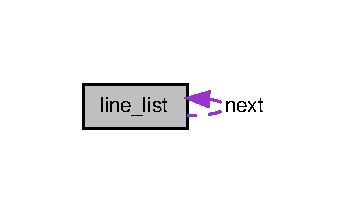
\includegraphics[width=167pt]{d9/df8/structline__list__coll__graph}
\end{center}
\end{figure}
\subsection*{Data Fields}
\begin{DoxyCompactItemize}
\item 
char $\ast$ {\bf string\_\-arg}
\item 
struct {\bf line\_\-list} $\ast$ {\bf next}
\end{DoxyCompactItemize}


\subsection{Field Documentation}
\index{line\_\-list@{line\_\-list}!next@{next}}
\index{next@{next}!line_list@{line\_\-list}}
\subsubsection[{next}]{\setlength{\rightskip}{0pt plus 5cm}struct {\bf line\_\-list}$\ast$ {\bf next}}\label{d8/dae/structline__list_ad41ea66e6cc047edbe477347cb73487d}
\index{line\_\-list@{line\_\-list}!string\_\-arg@{string\_\-arg}}
\index{string\_\-arg@{string\_\-arg}!line_list@{line\_\-list}}
\subsubsection[{string\_\-arg}]{\setlength{\rightskip}{0pt plus 5cm}char$\ast$ {\bf string\_\-arg}}\label{d8/dae/structline__list_a9a5dcb426087730237be62a9bf2f83f0}


The documentation for this struct was generated from the following file:\begin{DoxyCompactItemize}
\item 
{\bf params.c}\end{DoxyCompactItemize}

\chapter{File Documentation}
\section{debug.c File Reference}
\label{d1/d72/debug_8c}\index{debug.c@{debug.c}}


Fun��es de depura��o  


{\ttfamily \#include $<$stdio.h$>$}\par
{\ttfamily \#include $<$stdarg.h$>$}\par
{\ttfamily \#include $<$stdlib.h$>$}\par
{\ttfamily \#include $<$string.h$>$}\par
{\ttfamily \#include $<$errno.h$>$}\par
{\ttfamily \#include $<$netdb.h$>$}\par
{\ttfamily \#include \char`\"{}debug.h\char`\"{}}\par
Include dependency graph for debug.c:\nopagebreak
\begin{figure}[H]
\begin{center}
\leavevmode
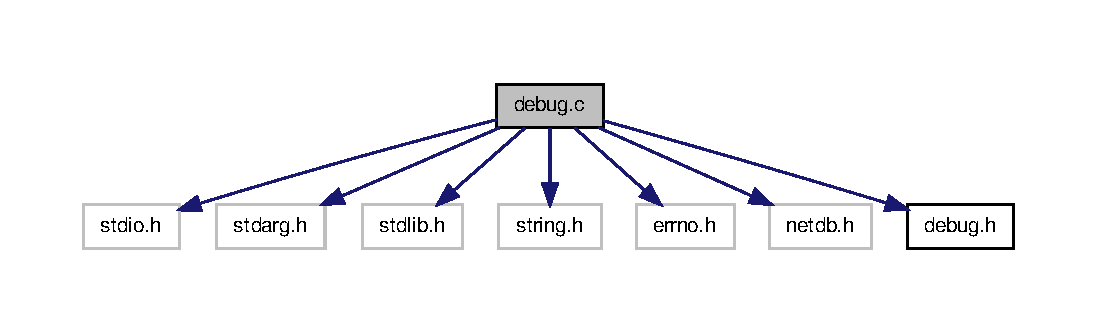
\includegraphics[width=400pt]{de/d23/debug_8c__incl}
\end{center}
\end{figure}
\subsection*{Functions}
\begin{DoxyCompactItemize}
\item 
void {\bf debug} (const char $\ast$file, const int line, char $\ast$fmt,...)
\item 
void {\bf warning} (const char $\ast$file, const int line, char $\ast$fmt,...)
\item 
void {\bf error} (const char $\ast$file, const int line, int exitCode, char $\ast$fmt,...)
\item 
void {\bf h\_\-warning} (const char $\ast$file, const int line, char $\ast$fmt,...)
\item 
void {\bf h\_\-error} (const char $\ast$file, const int line, int exitCode, char $\ast$fmt,...)
\end{DoxyCompactItemize}


\subsection{Detailed Description}
Fun��es de depura��o Fun��es de depura��o que ser�o chamadas atrav�s das respectivas macros definidas no ficheiro \doxyref{debug.h}{p.}{db/d16/debug_8h}. O objectivo destas fun��es � auxiliar o tratamento de erros e a depura��o

\begin{DoxyAuthor}{Author}
Miguel Frade, Patricio Domingues, Vitor Carreira 
\end{DoxyAuthor}
\begin{DoxyDate}{Date}
Agosto de 2003 
\end{DoxyDate}
\begin{DoxyVersion}{Version}
2 
\end{DoxyVersion}


\subsection{Function Documentation}
\index{debug.c@{debug.c}!debug@{debug}}
\index{debug@{debug}!debug.c@{debug.c}}
\subsubsection[{debug}]{\setlength{\rightskip}{0pt plus 5cm}void debug (
\begin{DoxyParamCaption}
\item[{const char $\ast$}]{file, }
\item[{const int}]{line, }
\item[{char $\ast$}]{fmt, }
\item[{}]{...}
\end{DoxyParamCaption}
)}\label{d1/d72/debug_8c_acc17bf1a6a66cde4a4b03e1376e68e20}
Esta fun��o deve ser utilizada para auxiliar a depura��o de programas. Esta fun��o {\bfseries n�o deve} ser chamada directamente, mas sim atrav�s da macro \doxyref{DEBUG()}{p.}{db/d16/debug_8h_a96dd473db0b3d10bd43390cdacb00120}.


\begin{DoxyParams}{Parameters}
{\em file} & nome do ficheiro (atrav�s da macro DEBUG) \\
\hline
{\em line} & linha onde a fun��o foi chamada (atrav�s da macro DEBUG) \\
\hline
{\em fmt} & string de formata��o como no \char`\"{}printf\char`\"{} \\
\hline
{\em ...} & n� vari�vel de par�metros \\
\hline
\end{DoxyParams}
\begin{DoxyReturn}{Returns}
A fun��o n�o retorna nada 
\end{DoxyReturn}
\begin{DoxySeeAlso}{See also}
\doxyref{DEBUG}{p.}{db/d16/debug_8h_a96dd473db0b3d10bd43390cdacb00120} 
\end{DoxySeeAlso}
\index{debug.c@{debug.c}!error@{error}}
\index{error@{error}!debug.c@{debug.c}}
\subsubsection[{error}]{\setlength{\rightskip}{0pt plus 5cm}void error (
\begin{DoxyParamCaption}
\item[{const char $\ast$}]{file, }
\item[{const int}]{line, }
\item[{int}]{exitCode, }
\item[{char $\ast$}]{fmt, }
\item[{}]{...}
\end{DoxyParamCaption}
)}\label{d1/d72/debug_8c_a00ba4f07a31f46cef16f3057b8662a96}
Fun��o que envia para o canal de erros a mensagem \char`\"{}ERROR\char`\"{} rotulada com o nome do ficheiro e da linha da fun��o chamante, e ainda da mensagem de erro do sistema. A fun��o {\bfseries n�o deve} ser chamada directamente, mas sim atrav�s da macro \doxyref{ERROR()}{p.}{db/d16/debug_8h_a8f448861da74111034b91e293ab3a278}.


\begin{DoxyParams}{Parameters}
{\em file} & nome do ficheiro fonte da fun��o chamante (atrav�s da macro ERROR) \\
\hline
{\em line} & linha onde a fun��o foi chamada (atrav�s da macro ERROR) \\
\hline
{\em exitCode} & valor passado � fun��o \char`\"{}exit()\char`\"{} \\
\hline
{\em fmt} & string de formata��o como no \char`\"{}printf\char`\"{} \\
\hline
{\em ...} & n� vari�vel de par�metros \\
\hline
\end{DoxyParams}
\begin{DoxyReturn}{Returns}
A fun��o n�o retorna nada 
\end{DoxyReturn}
\begin{DoxySeeAlso}{See also}
\doxyref{ERROR}{p.}{db/d16/debug_8h_a8f448861da74111034b91e293ab3a278} 
\end{DoxySeeAlso}
\index{debug.c@{debug.c}!h\_\-error@{h\_\-error}}
\index{h\_\-error@{h\_\-error}!debug.c@{debug.c}}
\subsubsection[{h\_\-error}]{\setlength{\rightskip}{0pt plus 5cm}void h\_\-error (
\begin{DoxyParamCaption}
\item[{const char $\ast$}]{file, }
\item[{const int}]{line, }
\item[{int}]{exitCode, }
\item[{char $\ast$}]{fmt, }
\item[{}]{...}
\end{DoxyParamCaption}
)}\label{d1/d72/debug_8c_ae9f36ff80fde369e5dc95cd100bcfb0d}
Fun��o que envia para o canal de erros a mensagem \char`\"{}H\_\-ERROR\char`\"{} rotulada com o nome do ficheiro e da linha da fun��o chamante, e ainda da mensagem de erro do sistema. A fun��o {\bfseries n�o deve} ser chamada directamente, mas sim atrav�s da macro \doxyref{H\_\-ERROR()}{p.}{db/d16/debug_8h_aa533515393a45f031c0841bb27e6f6ad}.


\begin{DoxyParams}{Parameters}
{\em file} & nome do ficheiro fonte da fun��o chamante (atrav�s da macro H\_\-ERROR) \\
\hline
{\em line} & linha onde a fun��o foi chamada (atrav�s da macro H\_\-ERROR) \\
\hline
{\em exitCode} & valor passado � fun��o \char`\"{}exit()\char`\"{} \\
\hline
{\em fmt} & string de formata��o como no \char`\"{}printf\char`\"{} \\
\hline
{\em ...} & n� vari�vel de par�metros \\
\hline
\end{DoxyParams}
\begin{DoxyReturn}{Returns}
A fun��o n�o retorna nada 
\end{DoxyReturn}
\begin{DoxySeeAlso}{See also}
\doxyref{H\_\-ERROR}{p.}{db/d16/debug_8h_aa533515393a45f031c0841bb27e6f6ad} 
\end{DoxySeeAlso}
\index{debug.c@{debug.c}!h\_\-warning@{h\_\-warning}}
\index{h\_\-warning@{h\_\-warning}!debug.c@{debug.c}}
\subsubsection[{h\_\-warning}]{\setlength{\rightskip}{0pt plus 5cm}void h\_\-warning (
\begin{DoxyParamCaption}
\item[{const char $\ast$}]{file, }
\item[{const int}]{line, }
\item[{char $\ast$}]{fmt, }
\item[{}]{...}
\end{DoxyParamCaption}
)}\label{d1/d72/debug_8c_aef70c8e59b9a71be54e6f859df15a183}
Fun��o que envia para o canal de erros a mensagem \char`\"{}H\_\-WARNING\char`\"{} rotulada com o nome do ficheiro e da linha da fun��o chamante, e ainda da mensagem de erro do sistema. A fun��o {\bfseries n�o deve} ser chamada directamente, mas sim atrav�s da macro \doxyref{H\_\-WARNING()}{p.}{db/d16/debug_8h_ada8f08bfa2fb4ed49f70f607b1673eca}.


\begin{DoxyParams}{Parameters}
{\em file} & nome do ficheiro fonte da fun��o chamante (atrav�s da macro H\_\-WARNING) \\
\hline
{\em line} & linha onde a fun��o foi chamada (atrav�s da macro H\_\-WARNING) \\
\hline
{\em fmt} & string de formata��o como no \char`\"{}printf\char`\"{} \\
\hline
{\em ...} & n� vari�vel de par�metros \\
\hline
\end{DoxyParams}
\begin{DoxyReturn}{Returns}
A fun��o n�o retorna nada 
\end{DoxyReturn}
\begin{DoxySeeAlso}{See also}
\doxyref{H\_\-WARNING}{p.}{db/d16/debug_8h_ada8f08bfa2fb4ed49f70f607b1673eca} 
\end{DoxySeeAlso}
\index{debug.c@{debug.c}!warning@{warning}}
\index{warning@{warning}!debug.c@{debug.c}}
\subsubsection[{warning}]{\setlength{\rightskip}{0pt plus 5cm}void warning (
\begin{DoxyParamCaption}
\item[{const char $\ast$}]{file, }
\item[{const int}]{line, }
\item[{char $\ast$}]{fmt, }
\item[{}]{...}
\end{DoxyParamCaption}
)}\label{d1/d72/debug_8c_a4befecaccba59492862dbf09c4c82b24}
Fun��o que envia para o canal de erros a mensagem \char`\"{}WARNING\char`\"{} rotulada com o nome do ficheiro e da linha da fun��o chamante e ainda da mensagem de erro do sistema. A fun��o {\bfseries n�o deve} ser chamada directamente, mas sim atrav�s da macro \doxyref{WARNING()}{p.}{db/d16/debug_8h_a8d12d0f11fc9acd2f1fa22d80895ddae}.


\begin{DoxyParams}{Parameters}
{\em file} & nome do ficheiro fonte da fun��o chamante (atrav�s da macro WARNING) \\
\hline
{\em line} & linha onde a fun��o foi chamada (atrav�s da macro WARNING) \\
\hline
{\em fmt} & string de formata��o como no \char`\"{}printf\char`\"{} \\
\hline
{\em ...} & n� vari�vel de par�metros \\
\hline
\end{DoxyParams}
\begin{DoxyReturn}{Returns}
A fun��o n�o retorna nada 
\end{DoxyReturn}
\begin{DoxySeeAlso}{See also}
\doxyref{WARNING}{p.}{db/d16/debug_8h_a8d12d0f11fc9acd2f1fa22d80895ddae} 
\end{DoxySeeAlso}

\section{debug.h File Reference}
\label{db/d16/debug_8h}\index{debug.h@{debug.h}}


Macros das fun��es de depura��o  


This graph shows which files directly or indirectly include this file:\nopagebreak
\begin{figure}[H]
\begin{center}
\leavevmode
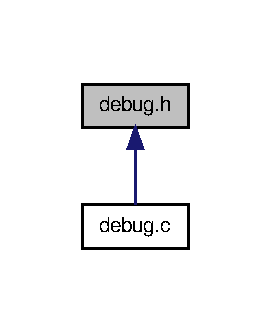
\includegraphics[width=130pt]{dc/dc8/debug_8h__dep__incl}
\end{center}
\end{figure}
\subsection*{Defines}
\begin{DoxyCompactItemize}
\item 
\#define {\bf DEBUG}(...)~debug(\_\-\_\-FILE\_\-\_\-, \_\-\_\-LINE\_\-\_\-, \_\-\_\-VA\_\-ARGS\_\-\_\-)
\item 
\#define {\bf WARNING}(...)~warning(\_\-\_\-FILE\_\-\_\-, \_\-\_\-LINE\_\-\_\-, \_\-\_\-VA\_\-ARGS\_\-\_\-)
\item 
\#define {\bf ERROR}(exitCode,...)~error(\_\-\_\-FILE\_\-\_\-, \_\-\_\-LINE\_\-\_\-, (exitCode), \_\-\_\-VA\_\-ARGS\_\-\_\-)
\item 
\#define {\bf H\_\-WARNING}(...)~h\_\-warning(\_\-\_\-FILE\_\-\_\-, \_\-\_\-LINE\_\-\_\-, \_\-\_\-VA\_\-ARGS\_\-\_\-)
\item 
\#define {\bf H\_\-ERROR}(exitCode,...)~h\_\-error(\_\-\_\-FILE\_\-\_\-, \_\-\_\-LINE\_\-\_\-, (exitCode), \_\-\_\-VA\_\-ARGS\_\-\_\-)
\end{DoxyCompactItemize}
\subsection*{Functions}
\begin{DoxyCompactItemize}
\item 
void {\bf debug} (const char $\ast$file, const int line, char $\ast$fmt,...)
\item 
void {\bf warning} (const char $\ast$file, const int line, char $\ast$fmt,...)
\item 
void {\bf error} (const char $\ast$file, const int line, int exitCode, char $\ast$fmt,...)
\item 
void {\bf h\_\-warning} (const char $\ast$file, const int line, char $\ast$fmt,...)
\item 
void {\bf h\_\-error} (const char $\ast$file, const int line, int exitCode, char $\ast$fmt,...)
\end{DoxyCompactItemize}


\subsection{Detailed Description}
Macros das fun��es de depura��o Macros que ser�o usadas nos programas desenvolvidos ao longo dos exemplos. Estas macros podem receber um n�mero vari�vel de par�metros atrav�s de uma string de formata��o como no \char`\"{}printf\char`\"{}. Seguem-\/se alguns exemplos: 
\begin{DoxyCode}
 DEBUG("i = %d e f=.2f%", i, f);
 ERROR("%s", msg);
\end{DoxyCode}
 \begin{DoxyAuthor}{Author}
Miguel Frade, Patricio Domingues, Vitor Carreira 
\end{DoxyAuthor}
\begin{DoxyDate}{Date}
Agosto de 2003 
\end{DoxyDate}
\begin{DoxyVersion}{Version}
2 
\end{DoxyVersion}


\subsection{Define Documentation}
\index{debug.h@{debug.h}!DEBUG@{DEBUG}}
\index{DEBUG@{DEBUG}!debug.h@{debug.h}}
\subsubsection[{DEBUG}]{\setlength{\rightskip}{0pt plus 5cm}\#define DEBUG(
\begin{DoxyParamCaption}
\item[{}]{...}
\end{DoxyParamCaption}
)~debug(\_\-\_\-FILE\_\-\_\-, \_\-\_\-LINE\_\-\_\-, \_\-\_\-VA\_\-ARGS\_\-\_\-)}\label{db/d16/debug_8h_a96dd473db0b3d10bd43390cdacb00120}
Macro para imprimir no stderr informa��es �teis para depura��o. O n�mero de par�metros de entrada � vari�vel.

\begin{DoxyReturn}{Returns}
A fun��o n�o retorna nada 
\end{DoxyReturn}
\begin{DoxySeeAlso}{See also}
\doxyref{debug()}{p.}{d1/d72/debug_8c_acc17bf1a6a66cde4a4b03e1376e68e20} 
\end{DoxySeeAlso}
\index{debug.h@{debug.h}!ERROR@{ERROR}}
\index{ERROR@{ERROR}!debug.h@{debug.h}}
\subsubsection[{ERROR}]{\setlength{\rightskip}{0pt plus 5cm}\#define ERROR(
\begin{DoxyParamCaption}
\item[{}]{exitCode, }
\item[{}]{...}
\end{DoxyParamCaption}
)~error(\_\-\_\-FILE\_\-\_\-, \_\-\_\-LINE\_\-\_\-, (exitCode), \_\-\_\-VA\_\-ARGS\_\-\_\-)}\label{db/d16/debug_8h_a8f448861da74111034b91e293ab3a278}
Macro para imprimir no stderr informa��o relacionada com insucesso de chamadas de fun��es e termina a execu��o do programa. O n�mero de par�metros de entrada � vari�vel.

\begin{DoxyReturn}{Returns}
A fun��o n�o retorna nada 
\end{DoxyReturn}
\begin{DoxySeeAlso}{See also}
\doxyref{error()}{p.}{d1/d72/debug_8c_a00ba4f07a31f46cef16f3057b8662a96} 
\end{DoxySeeAlso}
\index{debug.h@{debug.h}!H\_\-ERROR@{H\_\-ERROR}}
\index{H\_\-ERROR@{H\_\-ERROR}!debug.h@{debug.h}}
\subsubsection[{H\_\-ERROR}]{\setlength{\rightskip}{0pt plus 5cm}\#define H\_\-ERROR(
\begin{DoxyParamCaption}
\item[{}]{exitCode, }
\item[{}]{...}
\end{DoxyParamCaption}
)~h\_\-error(\_\-\_\-FILE\_\-\_\-, \_\-\_\-LINE\_\-\_\-, (exitCode), \_\-\_\-VA\_\-ARGS\_\-\_\-)}\label{db/d16/debug_8h_aa533515393a45f031c0841bb27e6f6ad}
Macro para imprimir no stderr informa��o relacionada com insucesso de chamadas de fun��es de resolu��o de nomes e termina a execu��o do programa. O n�mero de par�metros de entrada � vari�vel.

\begin{DoxyReturn}{Returns}
A fun��o n�o retorna nada 
\end{DoxyReturn}
\begin{DoxySeeAlso}{See also}
\doxyref{h\_\-error()}{p.}{d1/d72/debug_8c_ae9f36ff80fde369e5dc95cd100bcfb0d} 
\end{DoxySeeAlso}
\index{debug.h@{debug.h}!H\_\-WARNING@{H\_\-WARNING}}
\index{H\_\-WARNING@{H\_\-WARNING}!debug.h@{debug.h}}
\subsubsection[{H\_\-WARNING}]{\setlength{\rightskip}{0pt plus 5cm}\#define H\_\-WARNING(
\begin{DoxyParamCaption}
\item[{}]{...}
\end{DoxyParamCaption}
)~h\_\-warning(\_\-\_\-FILE\_\-\_\-, \_\-\_\-LINE\_\-\_\-, \_\-\_\-VA\_\-ARGS\_\-\_\-)}\label{db/d16/debug_8h_ada8f08bfa2fb4ed49f70f607b1673eca}
Macro para imprimir no stderr informa��o relacionada com insucesso de chamadas de fun��es de resolu��o de nomes, mas n�o termina a execu��o do programa. O n�mero de par�metros de entrada � vari�vel.

\begin{DoxyReturn}{Returns}
A fun��o n�o retorna nada 
\end{DoxyReturn}
\begin{DoxySeeAlso}{See also}
\doxyref{h\_\-warning()}{p.}{d1/d72/debug_8c_aef70c8e59b9a71be54e6f859df15a183} 
\end{DoxySeeAlso}
\index{debug.h@{debug.h}!WARNING@{WARNING}}
\index{WARNING@{WARNING}!debug.h@{debug.h}}
\subsubsection[{WARNING}]{\setlength{\rightskip}{0pt plus 5cm}\#define WARNING(
\begin{DoxyParamCaption}
\item[{}]{...}
\end{DoxyParamCaption}
)~warning(\_\-\_\-FILE\_\-\_\-, \_\-\_\-LINE\_\-\_\-, \_\-\_\-VA\_\-ARGS\_\-\_\-)}\label{db/d16/debug_8h_a8d12d0f11fc9acd2f1fa22d80895ddae}
Macro para imprimir no stderr informa��o relacionada com insucesso de chamadas de fun��es, mas n�o termina a execu��o do programa. O n�mero de par�metros de entrada � vari�vel.

\begin{DoxyReturn}{Returns}
A fun��o n�o retorna nada 
\end{DoxyReturn}
\begin{DoxySeeAlso}{See also}
\doxyref{warning()}{p.}{d1/d72/debug_8c_a4befecaccba59492862dbf09c4c82b24} 
\end{DoxySeeAlso}


\subsection{Function Documentation}
\index{debug.h@{debug.h}!debug@{debug}}
\index{debug@{debug}!debug.h@{debug.h}}
\subsubsection[{debug}]{\setlength{\rightskip}{0pt plus 5cm}void debug (
\begin{DoxyParamCaption}
\item[{const char $\ast$}]{file, }
\item[{const int}]{line, }
\item[{char $\ast$}]{fmt, }
\item[{}]{...}
\end{DoxyParamCaption}
)}\label{db/d16/debug_8h_acc17bf1a6a66cde4a4b03e1376e68e20}
Esta fun��o deve ser utilizada para auxiliar a depura��o de programas. Esta fun��o {\bfseries n�o deve} ser chamada directamente, mas sim atrav�s da macro \doxyref{DEBUG()}{p.}{db/d16/debug_8h_a96dd473db0b3d10bd43390cdacb00120}.


\begin{DoxyParams}{Parameters}
{\em file} & nome do ficheiro (atrav�s da macro DEBUG) \\
\hline
{\em line} & linha onde a fun��o foi chamada (atrav�s da macro DEBUG) \\
\hline
{\em fmt} & string de formata��o como no \char`\"{}printf\char`\"{} \\
\hline
{\em ...} & n� vari�vel de par�metros \\
\hline
\end{DoxyParams}
\begin{DoxyReturn}{Returns}
A fun��o n�o retorna nada 
\end{DoxyReturn}
\begin{DoxySeeAlso}{See also}
\doxyref{DEBUG}{p.}{db/d16/debug_8h_a96dd473db0b3d10bd43390cdacb00120} 
\end{DoxySeeAlso}
\index{debug.h@{debug.h}!error@{error}}
\index{error@{error}!debug.h@{debug.h}}
\subsubsection[{error}]{\setlength{\rightskip}{0pt plus 5cm}void error (
\begin{DoxyParamCaption}
\item[{const char $\ast$}]{file, }
\item[{const int}]{line, }
\item[{int}]{exitCode, }
\item[{char $\ast$}]{fmt, }
\item[{}]{...}
\end{DoxyParamCaption}
)}\label{db/d16/debug_8h_a00ba4f07a31f46cef16f3057b8662a96}
Fun��o que envia para o canal de erros a mensagem \char`\"{}ERROR\char`\"{} rotulada com o nome do ficheiro e da linha da fun��o chamante, e ainda da mensagem de erro do sistema. A fun��o {\bfseries n�o deve} ser chamada directamente, mas sim atrav�s da macro \doxyref{ERROR()}{p.}{db/d16/debug_8h_a8f448861da74111034b91e293ab3a278}.


\begin{DoxyParams}{Parameters}
{\em file} & nome do ficheiro fonte da fun��o chamante (atrav�s da macro ERROR) \\
\hline
{\em line} & linha onde a fun��o foi chamada (atrav�s da macro ERROR) \\
\hline
{\em exitCode} & valor passado � fun��o \char`\"{}exit()\char`\"{} \\
\hline
{\em fmt} & string de formata��o como no \char`\"{}printf\char`\"{} \\
\hline
{\em ...} & n� vari�vel de par�metros \\
\hline
\end{DoxyParams}
\begin{DoxyReturn}{Returns}
A fun��o n�o retorna nada 
\end{DoxyReturn}
\begin{DoxySeeAlso}{See also}
\doxyref{ERROR}{p.}{db/d16/debug_8h_a8f448861da74111034b91e293ab3a278} 
\end{DoxySeeAlso}
\index{debug.h@{debug.h}!h\_\-error@{h\_\-error}}
\index{h\_\-error@{h\_\-error}!debug.h@{debug.h}}
\subsubsection[{h\_\-error}]{\setlength{\rightskip}{0pt plus 5cm}void h\_\-error (
\begin{DoxyParamCaption}
\item[{const char $\ast$}]{file, }
\item[{const int}]{line, }
\item[{int}]{exitCode, }
\item[{char $\ast$}]{fmt, }
\item[{}]{...}
\end{DoxyParamCaption}
)}\label{db/d16/debug_8h_ae9f36ff80fde369e5dc95cd100bcfb0d}
Fun��o que envia para o canal de erros a mensagem \char`\"{}H\_\-ERROR\char`\"{} rotulada com o nome do ficheiro e da linha da fun��o chamante, e ainda da mensagem de erro do sistema. A fun��o {\bfseries n�o deve} ser chamada directamente, mas sim atrav�s da macro \doxyref{H\_\-ERROR()}{p.}{db/d16/debug_8h_aa533515393a45f031c0841bb27e6f6ad}.


\begin{DoxyParams}{Parameters}
{\em file} & nome do ficheiro fonte da fun��o chamante (atrav�s da macro H\_\-ERROR) \\
\hline
{\em line} & linha onde a fun��o foi chamada (atrav�s da macro H\_\-ERROR) \\
\hline
{\em exitCode} & valor passado � fun��o \char`\"{}exit()\char`\"{} \\
\hline
{\em fmt} & string de formata��o como no \char`\"{}printf\char`\"{} \\
\hline
{\em ...} & n� vari�vel de par�metros \\
\hline
\end{DoxyParams}
\begin{DoxyReturn}{Returns}
A fun��o n�o retorna nada 
\end{DoxyReturn}
\begin{DoxySeeAlso}{See also}
\doxyref{H\_\-ERROR}{p.}{db/d16/debug_8h_aa533515393a45f031c0841bb27e6f6ad} 
\end{DoxySeeAlso}
\index{debug.h@{debug.h}!h\_\-warning@{h\_\-warning}}
\index{h\_\-warning@{h\_\-warning}!debug.h@{debug.h}}
\subsubsection[{h\_\-warning}]{\setlength{\rightskip}{0pt plus 5cm}void h\_\-warning (
\begin{DoxyParamCaption}
\item[{const char $\ast$}]{file, }
\item[{const int}]{line, }
\item[{char $\ast$}]{fmt, }
\item[{}]{...}
\end{DoxyParamCaption}
)}\label{db/d16/debug_8h_aef70c8e59b9a71be54e6f859df15a183}
Fun��o que envia para o canal de erros a mensagem \char`\"{}H\_\-WARNING\char`\"{} rotulada com o nome do ficheiro e da linha da fun��o chamante, e ainda da mensagem de erro do sistema. A fun��o {\bfseries n�o deve} ser chamada directamente, mas sim atrav�s da macro \doxyref{H\_\-WARNING()}{p.}{db/d16/debug_8h_ada8f08bfa2fb4ed49f70f607b1673eca}.


\begin{DoxyParams}{Parameters}
{\em file} & nome do ficheiro fonte da fun��o chamante (atrav�s da macro H\_\-WARNING) \\
\hline
{\em line} & linha onde a fun��o foi chamada (atrav�s da macro H\_\-WARNING) \\
\hline
{\em fmt} & string de formata��o como no \char`\"{}printf\char`\"{} \\
\hline
{\em ...} & n� vari�vel de par�metros \\
\hline
\end{DoxyParams}
\begin{DoxyReturn}{Returns}
A fun��o n�o retorna nada 
\end{DoxyReturn}
\begin{DoxySeeAlso}{See also}
\doxyref{H\_\-WARNING}{p.}{db/d16/debug_8h_ada8f08bfa2fb4ed49f70f607b1673eca} 
\end{DoxySeeAlso}
\index{debug.h@{debug.h}!warning@{warning}}
\index{warning@{warning}!debug.h@{debug.h}}
\subsubsection[{warning}]{\setlength{\rightskip}{0pt plus 5cm}void warning (
\begin{DoxyParamCaption}
\item[{const char $\ast$}]{file, }
\item[{const int}]{line, }
\item[{char $\ast$}]{fmt, }
\item[{}]{...}
\end{DoxyParamCaption}
)}\label{db/d16/debug_8h_a4befecaccba59492862dbf09c4c82b24}
Fun��o que envia para o canal de erros a mensagem \char`\"{}WARNING\char`\"{} rotulada com o nome do ficheiro e da linha da fun��o chamante e ainda da mensagem de erro do sistema. A fun��o {\bfseries n�o deve} ser chamada directamente, mas sim atrav�s da macro \doxyref{WARNING()}{p.}{db/d16/debug_8h_a8d12d0f11fc9acd2f1fa22d80895ddae}.


\begin{DoxyParams}{Parameters}
{\em file} & nome do ficheiro fonte da fun��o chamante (atrav�s da macro WARNING) \\
\hline
{\em line} & linha onde a fun��o foi chamada (atrav�s da macro WARNING) \\
\hline
{\em fmt} & string de formata��o como no \char`\"{}printf\char`\"{} \\
\hline
{\em ...} & n� vari�vel de par�metros \\
\hline
\end{DoxyParams}
\begin{DoxyReturn}{Returns}
A fun��o n�o retorna nada 
\end{DoxyReturn}
\begin{DoxySeeAlso}{See also}
\doxyref{WARNING}{p.}{db/d16/debug_8h_a8d12d0f11fc9acd2f1fa22d80895ddae} 
\end{DoxySeeAlso}

\section{main.c File Reference}
\label{d0/d29/main_8c}\index{main.c@{main.c}}
{\ttfamily \#include $<$stdio.h$>$}\par
{\ttfamily \#include $<$stdlib.h$>$}\par
{\ttfamily \#include $<$math.h$>$}\par
{\ttfamily \#include $<$float.h$>$}\par
{\ttfamily \#include $<$string.h$>$}\par
{\ttfamily \#include $<$unistd.h$>$}\par
{\ttfamily \#include $<$ctype.h$>$}\par
{\ttfamily \#include $<$time.h$>$}\par
{\ttfamily \#include $<$sys/types.h$>$}\par
{\ttfamily \#include $<$sys/stat.h$>$}\par
{\ttfamily \#include $<$fcntl.h$>$}\par
{\ttfamily \#include \char`\"{}params.h\char`\"{}}\par
Include dependency graph for main.c:\nopagebreak
\begin{figure}[H]
\begin{center}
\leavevmode
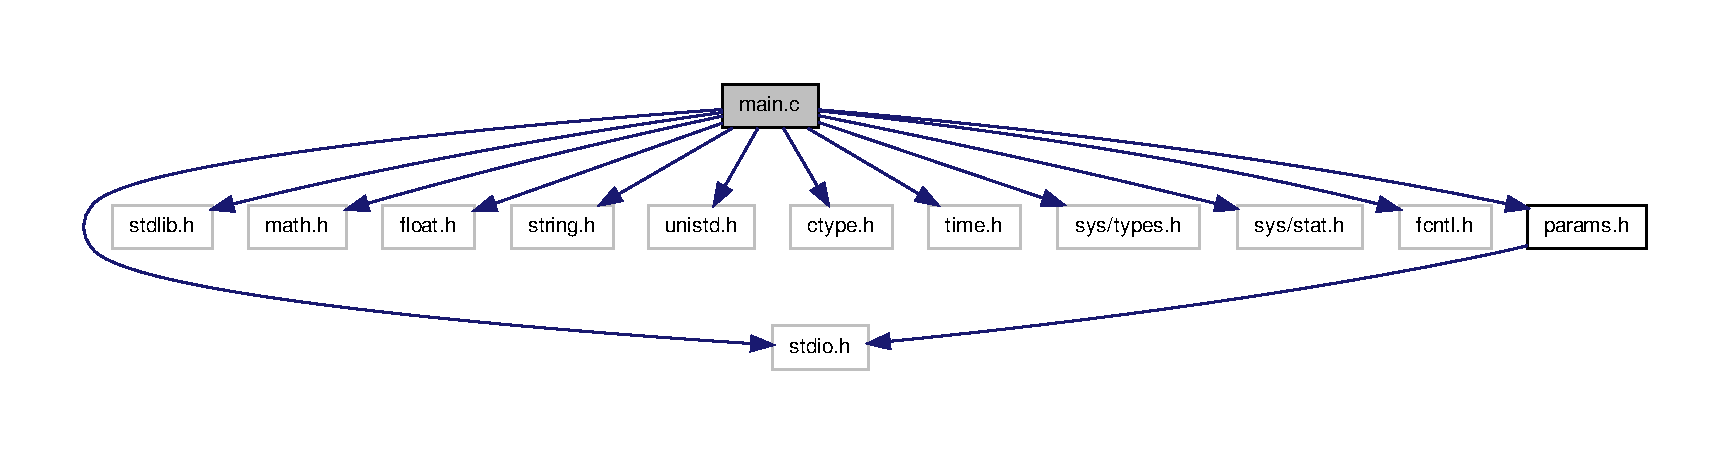
\includegraphics[width=400pt]{d4/d10/main_8c__incl}
\end{center}
\end{figure}
\subsection*{Defines}
\begin{DoxyCompactItemize}
\item 
\#define {\bf ERROR\_\-INVALID\_\-PARAMETERS}~1
\begin{DoxyCompactList}\small\item\em $\ast$/ \end{DoxyCompactList}\item 
\#define {\bf ERROR\_\-ALLOCATE\_\-MEMORY}~2
\item 
\#define {\bf ERROR\_\-OPEN\_\-FILE}
\item 
\#define {\bf ERROR\_\-INVALID\_\-PARAMETERS}~1
\begin{DoxyCompactList}\small\item\em $\ast$/ \end{DoxyCompactList}\item 
\#define {\bf RANGE\_\-LUMINANCE}~255
\begin{DoxyCompactList}\small\item\em $\ast$$\ast$$\ast$$\ast$$\ast$$\ast$$\ast$$\ast$$\ast$$\ast$$\ast$$\ast$$\ast$$\ast$$\ast$$\ast$$\ast$$\ast$$\ast$ END CONSTANTES ERROR DEFINITION $\ast$$\ast$$\ast$$\ast$$\ast$$\ast$$\ast$$\ast$$\ast$$\ast$$\ast$$\ast$$\ast$$\ast$$\ast$$\ast$$\ast$$\ast$$\ast$$\ast$$\ast$$\ast$/// \end{DoxyCompactList}\item 
\#define {\bf PERMS}~0644
\item 
\#define {\bf RANGEY}~255
\item 
\#define {\bf Clip1}(a)~((a)$>$255?255:((a)$<$0?0:(a)))
\end{DoxyCompactItemize}
\subsection*{Functions}
\begin{DoxyCompactItemize}
\item 
void {\bf read\_\-header\_\-pgm} (int $\ast$ysize, int $\ast$xsize, char $\ast$file\_\-name)
\begin{DoxyCompactList}\small\item\em $\ast$$\ast$$\ast$$\ast$$\ast$$\ast$$\ast$$\ast$$\ast$$\ast$$\ast$$\ast$$\ast$$\ast$$\ast$$\ast$$\ast$$\ast$$\ast$$\ast$$\ast$$\ast$$\ast$$\ast$ END CONSTANTES DEFINITION $\ast$$\ast$$\ast$$\ast$$\ast$$\ast$$\ast$$\ast$$\ast$$\ast$$\ast$$\ast$$\ast$$\ast$$\ast$$\ast$$\ast$$\ast$$\ast$$\ast$$\ast$$\ast$$\ast$/// \end{DoxyCompactList}\item 
void {\bf read\_\-file\_\-pgm} (int $\ast$$\ast$pelimg, int $\ast$ysize, int $\ast$xsize, char $\ast$file\_\-name)
\item 
void {\bf v\_\-read\_\-file\_\-pgm} (int $\ast$pelimg, int $\ast$ysize, int $\ast$xsize, char $\ast$file\_\-name)
\item 
int $\ast$$\ast$ {\bf int\_\-matrix} (int nr, int nc)
\item 
float $\ast$$\ast$ {\bf floatmatrix} (int nr, int nc)
\item 
int $\ast$ {\bf int\_\-vector} (int nr, int nc)
\item 
float {\bf quad\_\-err} (int index\_\-dic, int $\ast$block\_\-size\_\-x, int $\ast$block\_\-size\_\-y, int $\ast$original\_\-block)
\item 
void {\bf load\_\-dictionary} (char $\ast$file\_\-name, int $\ast$num\_\-codewords, int $\ast$block\_\-size\_\-x, int $\ast$block\_\-size\_\-y)
\item 
double {\bf calculate\_\-psnr} (int $\ast$$\ast$origblk, int $\ast$$\ast$cmpblk, int nline, int npixel)
\item 
double {\bf calculate\_\-mse} (int $\ast$$\ast$origblk, int $\ast$$\ast$cmpblk, int nline, int npixel)
\item 
void {\bf write\_\-index} (int index, int bits\_\-index, long $\ast$bits\_\-count, int $\ast$bits\_\-to\_\-go, int $\ast$buffer, FILE $\ast$pointf\_\-out)
\item 
void {\bf write\_\-f\_\-pgm} (int $\ast$$\ast$im\_\-matrix, int nline, int npixel, char $\ast$filename)
\item 
unsigned char $\ast$$\ast$ {\bf ucmatrix} (int nrl, int nrh, int ncl, int nch)
\item 
void {\bf output\_\-bit} (int bit, FILE $\ast$output\_\-file, int $\ast$buffer, int $\ast$bits\_\-to\_\-go, long $\ast$bits\_\-count)
\item 
void {\bf done\_\-outputing\_\-bits} (FILE $\ast$output\_\-file, int $\ast$buffer, int $\ast$bits\_\-to\_\-go)
\item 
int {\bf main} (int argc, char $\ast$argv[$\,$])
\end{DoxyCompactItemize}
\subsection*{Variables}
\begin{DoxyCompactItemize}
\item 
$\ast$GLOBAL VARIABLES $\ast$$\ast$$\ast$$\ast$$\ast$$\ast$$\ast$$\ast$$\ast$$\ast$$\ast$$\ast$$\ast$$\ast$$\ast$$\ast$$\ast$$\ast$$\ast$$\ast$$\ast$$\ast$$\ast$$\ast$$\ast$$\ast$$\ast$$\ast$$\ast$$\ast$$\ast$$\ast$$\ast$$\ast$$\ast$$\ast$$\ast$$\ast$$\ast$$\ast$$\ast$$\ast$$\ast$$\ast$$\ast$$\ast$$\ast$$\ast$$\ast$$\ast$$\ast$$\ast$$\ast$$\ast$$\ast$$\ast$$\ast$$\ast$$\ast$$\ast$$\ast$$\ast$$\ast$$\ast$$\ast$$\ast$$\ast$$\ast$$\ast$$\ast$$\ast$$\ast$$\ast$$\ast$$\ast$int {\bf G\_\-dic}
\begin{DoxyCompactList}\small\item\em $\ast$$\ast$$\ast$$\ast$$\ast$$\ast$$\ast$$\ast$$\ast$$\ast$$\ast$$\ast$$\ast$$\ast$$\ast$$\ast$$\ast$$\ast$$\ast$$\ast$$\ast$$\ast$$\ast$$\ast$ END PROTOTYPES DEFINITION $\ast$$\ast$$\ast$$\ast$$\ast$$\ast$$\ast$$\ast$$\ast$$\ast$$\ast$$\ast$$\ast$$\ast$$\ast$$\ast$$\ast$$\ast$$\ast$$\ast$$\ast$$\ast$$\ast$/// \end{DoxyCompactList}\end{DoxyCompactItemize}


\subsection{Define Documentation}
\index{main.c@{main.c}!Clip1@{Clip1}}
\index{Clip1@{Clip1}!main.c@{main.c}}
\subsubsection[{Clip1}]{\setlength{\rightskip}{0pt plus 5cm}\#define Clip1(
\begin{DoxyParamCaption}
\item[{}]{a}
\end{DoxyParamCaption}
)~((a)$>$255?255:((a)$<$0?0:(a)))}\label{d0/d29/main_8c_ae16749d1d534e8f6ed34befc002309fe}
\index{main.c@{main.c}!ERROR\_\-ALLOCATE\_\-MEMORY@{ERROR\_\-ALLOCATE\_\-MEMORY}}
\index{ERROR\_\-ALLOCATE\_\-MEMORY@{ERROR\_\-ALLOCATE\_\-MEMORY}!main.c@{main.c}}
\subsubsection[{ERROR\_\-ALLOCATE\_\-MEMORY}]{\setlength{\rightskip}{0pt plus 5cm}\#define ERROR\_\-ALLOCATE\_\-MEMORY~2}\label{d0/d29/main_8c_ad0ad26cfa67e14427a22fcacad88aec4}
\index{main.c@{main.c}!ERROR\_\-INVALID\_\-PARAMETERS@{ERROR\_\-INVALID\_\-PARAMETERS}}
\index{ERROR\_\-INVALID\_\-PARAMETERS@{ERROR\_\-INVALID\_\-PARAMETERS}!main.c@{main.c}}
\subsubsection[{ERROR\_\-INVALID\_\-PARAMETERS}]{\setlength{\rightskip}{0pt plus 5cm}\#define ERROR\_\-INVALID\_\-PARAMETERS~1}\label{d0/d29/main_8c_a7656f0e76a5a4f4aa72fcb0afc3a2298}


$\ast$/ 

\index{main.c@{main.c}!ERROR\_\-INVALID\_\-PARAMETERS@{ERROR\_\-INVALID\_\-PARAMETERS}}
\index{ERROR\_\-INVALID\_\-PARAMETERS@{ERROR\_\-INVALID\_\-PARAMETERS}!main.c@{main.c}}
\subsubsection[{ERROR\_\-INVALID\_\-PARAMETERS}]{\setlength{\rightskip}{0pt plus 5cm}\#define ERROR\_\-INVALID\_\-PARAMETERS~1}\label{d0/d29/main_8c_a7656f0e76a5a4f4aa72fcb0afc3a2298}


$\ast$/ 

\index{main.c@{main.c}!ERROR\_\-OPEN\_\-FILE@{ERROR\_\-OPEN\_\-FILE}}
\index{ERROR\_\-OPEN\_\-FILE@{ERROR\_\-OPEN\_\-FILE}!main.c@{main.c}}
\subsubsection[{ERROR\_\-OPEN\_\-FILE}]{\setlength{\rightskip}{0pt plus 5cm}\#define ERROR\_\-OPEN\_\-FILE}\label{d0/d29/main_8c_a18acdce401ee0e52073166b285b3c56e}
\index{main.c@{main.c}!PERMS@{PERMS}}
\index{PERMS@{PERMS}!main.c@{main.c}}
\subsubsection[{PERMS}]{\setlength{\rightskip}{0pt plus 5cm}\#define PERMS~0644}\label{d0/d29/main_8c_afee0dce2271f56a18b4656548b2de8cc}
\index{main.c@{main.c}!RANGE\_\-LUMINANCE@{RANGE\_\-LUMINANCE}}
\index{RANGE\_\-LUMINANCE@{RANGE\_\-LUMINANCE}!main.c@{main.c}}
\subsubsection[{RANGE\_\-LUMINANCE}]{\setlength{\rightskip}{0pt plus 5cm}\#define RANGE\_\-LUMINANCE~255}\label{d0/d29/main_8c_a027288799bd249e133a0cd507fb2f08b}


$\ast$$\ast$$\ast$$\ast$$\ast$$\ast$$\ast$$\ast$$\ast$$\ast$$\ast$$\ast$$\ast$$\ast$$\ast$$\ast$$\ast$$\ast$$\ast$ END CONSTANTES ERROR DEFINITION $\ast$$\ast$$\ast$$\ast$$\ast$$\ast$$\ast$$\ast$$\ast$$\ast$$\ast$$\ast$$\ast$$\ast$$\ast$$\ast$$\ast$$\ast$$\ast$$\ast$$\ast$$\ast$/// 

$\ast$/ \index{main.c@{main.c}!RANGEY@{RANGEY}}
\index{RANGEY@{RANGEY}!main.c@{main.c}}
\subsubsection[{RANGEY}]{\setlength{\rightskip}{0pt plus 5cm}\#define RANGEY~255}\label{d0/d29/main_8c_a39c65b7495b2817cd8b49bd7acb5f2d2}


\subsection{Function Documentation}
\index{main.c@{main.c}!calculate\_\-mse@{calculate\_\-mse}}
\index{calculate\_\-mse@{calculate\_\-mse}!main.c@{main.c}}
\subsubsection[{calculate\_\-mse}]{\setlength{\rightskip}{0pt plus 5cm}double calculate\_\-mse (
\begin{DoxyParamCaption}
\item[{int $\ast$$\ast$}]{origblk, }
\item[{int $\ast$$\ast$}]{cmpblk, }
\item[{int}]{nline, }
\item[{int}]{npixel}
\end{DoxyParamCaption}
)}\label{d0/d29/main_8c_ad5b31f279c0814b74e3c2debdd0dc1c4}
\index{main.c@{main.c}!calculate\_\-psnr@{calculate\_\-psnr}}
\index{calculate\_\-psnr@{calculate\_\-psnr}!main.c@{main.c}}
\subsubsection[{calculate\_\-psnr}]{\setlength{\rightskip}{0pt plus 5cm}double calculate\_\-psnr (
\begin{DoxyParamCaption}
\item[{int $\ast$$\ast$}]{origblk, }
\item[{int $\ast$$\ast$}]{cmpblk, }
\item[{int}]{nline, }
\item[{int}]{npixel}
\end{DoxyParamCaption}
)}\label{d0/d29/main_8c_a656b25401cf282298f26c590fb6ae7f6}
\index{main.c@{main.c}!done\_\-outputing\_\-bits@{done\_\-outputing\_\-bits}}
\index{done\_\-outputing\_\-bits@{done\_\-outputing\_\-bits}!main.c@{main.c}}
\subsubsection[{done\_\-outputing\_\-bits}]{\setlength{\rightskip}{0pt plus 5cm}void done\_\-outputing\_\-bits (
\begin{DoxyParamCaption}
\item[{FILE $\ast$}]{output\_\-file, }
\item[{int $\ast$}]{buffer, }
\item[{int $\ast$}]{bits\_\-to\_\-go}
\end{DoxyParamCaption}
)}\label{d0/d29/main_8c_a19bc4ab525c95829e4991780228ffa65}
\index{main.c@{main.c}!floatmatrix@{floatmatrix}}
\index{floatmatrix@{floatmatrix}!main.c@{main.c}}
\subsubsection[{floatmatrix}]{\setlength{\rightskip}{0pt plus 5cm}float $\ast$$\ast$ floatmatrix (
\begin{DoxyParamCaption}
\item[{int}]{nr, }
\item[{int}]{nc}
\end{DoxyParamCaption}
)}\label{d0/d29/main_8c_a6d41dea8b750e37c064b4fda82331415}
Allocates memory for a matrix of variables of type float. 


\begin{DoxyParams}{Parameters}
{\em nr} & number of rows \\
\hline
{\em nc} & number of columns \\
\hline
\end{DoxyParams}
\begin{DoxyReturn}{Returns}
a pointer to a int matrix (float $\ast$$\ast$) 
\end{DoxyReturn}
\index{main.c@{main.c}!int\_\-matrix@{int\_\-matrix}}
\index{int\_\-matrix@{int\_\-matrix}!main.c@{main.c}}
\subsubsection[{int\_\-matrix}]{\setlength{\rightskip}{0pt plus 5cm}int $\ast$$\ast$ int\_\-matrix (
\begin{DoxyParamCaption}
\item[{int}]{nr, }
\item[{int}]{nc}
\end{DoxyParamCaption}
)}\label{d0/d29/main_8c_adea1cfc11f2b856be9fdeee0448edde5}
Allocates memory for a matrix of variables of type int. 


\begin{DoxyParams}{Parameters}
{\em nr} & number of rows \\
\hline
{\em nc} & number of columns \\
\hline
\end{DoxyParams}
\begin{DoxyReturn}{Returns}
a pointer to a int matrix (int $\ast$$\ast$) 
\end{DoxyReturn}
\index{main.c@{main.c}!int\_\-vector@{int\_\-vector}}
\index{int\_\-vector@{int\_\-vector}!main.c@{main.c}}
\subsubsection[{int\_\-vector}]{\setlength{\rightskip}{0pt plus 5cm}int $\ast$ int\_\-vector (
\begin{DoxyParamCaption}
\item[{int}]{nr, }
\item[{int}]{nc}
\end{DoxyParamCaption}
)}\label{d0/d29/main_8c_ab67cfb420c7a550017d13d7c3667c4c0}
Allocates memory for a vector of variables of type int. 


\begin{DoxyParams}{Parameters}
{\em nr} & number of rows \\
\hline
{\em nc} & number of columns \\
\hline
\end{DoxyParams}
\begin{DoxyReturn}{Returns}
a pointer to a int vector (int $\ast$) 
\end{DoxyReturn}
\index{main.c@{main.c}!load\_\-dictionary@{load\_\-dictionary}}
\index{load\_\-dictionary@{load\_\-dictionary}!main.c@{main.c}}
\subsubsection[{load\_\-dictionary}]{\setlength{\rightskip}{0pt plus 5cm}void load\_\-dictionary (
\begin{DoxyParamCaption}
\item[{char $\ast$}]{file\_\-name, }
\item[{int $\ast$}]{num\_\-codewords, }
\item[{int $\ast$}]{block\_\-size\_\-x, }
\item[{int $\ast$}]{block\_\-size\_\-y}
\end{DoxyParamCaption}
)}\label{d0/d29/main_8c_ab8fcf16cdfee7d4b099a8689b0ec5c2a}
Load the dictionary file to memory. 


\begin{DoxyParams}{Parameters}
{\em file\_\-name} & the name of the dictionary file \\
\hline
{\em num\_\-codewords} & number of blocks of the dictionary \\
\hline
{\em block\_\-size\_\-x} & horizontal size of the block \\
\hline
{\em block\_\-size\_\-y} & vertical size of the block \\
\hline
\end{DoxyParams}
\index{main.c@{main.c}!main@{main}}
\index{main@{main}!main.c@{main.c}}
\subsubsection[{main}]{\setlength{\rightskip}{0pt plus 5cm}int main (
\begin{DoxyParamCaption}
\item[{int}]{argc, }
\item[{char $\ast$}]{argv[$\,$]}
\end{DoxyParamCaption}
)}\label{d0/d29/main_8c_a0ddf1224851353fc92bfbff6f499fa97}
\index{main.c@{main.c}!output\_\-bit@{output\_\-bit}}
\index{output\_\-bit@{output\_\-bit}!main.c@{main.c}}
\subsubsection[{output\_\-bit}]{\setlength{\rightskip}{0pt plus 5cm}void output\_\-bit (
\begin{DoxyParamCaption}
\item[{int}]{bit, }
\item[{FILE $\ast$}]{output\_\-file, }
\item[{int $\ast$}]{buffer, }
\item[{int $\ast$}]{bits\_\-to\_\-go, }
\item[{long $\ast$}]{bits\_\-count}
\end{DoxyParamCaption}
)}\label{d0/d29/main_8c_a03d3bbe2b08e8abcd1f1e951220221f6}
\index{main.c@{main.c}!quad\_\-err@{quad\_\-err}}
\index{quad\_\-err@{quad\_\-err}!main.c@{main.c}}
\subsubsection[{quad\_\-err}]{\setlength{\rightskip}{0pt plus 5cm}float quad\_\-err (
\begin{DoxyParamCaption}
\item[{int}]{index\_\-dic, }
\item[{int $\ast$}]{block\_\-size\_\-x, }
\item[{int $\ast$}]{block\_\-size\_\-y, }
\item[{int $\ast$}]{original\_\-block}
\end{DoxyParamCaption}
)}\label{d0/d29/main_8c_a4c5537382802ddd75a4692945b1acd14}
Calculate the square error between a vector and a training set of the codebook vector. 


\begin{DoxyParams}{Parameters}
{\em index\_\-dic} & index of the dictionary row \\
\hline
{\em block\_\-size\_\-x} & horizontal size of the block \\
\hline
{\em block\_\-size\_\-y} & vertical size of the block \\
\hline
{\em original\_\-block} & the current block \\
\hline
\end{DoxyParams}
\begin{DoxyReturn}{Returns}
the square error value 
\end{DoxyReturn}
\index{main.c@{main.c}!read\_\-file\_\-pgm@{read\_\-file\_\-pgm}}
\index{read\_\-file\_\-pgm@{read\_\-file\_\-pgm}!main.c@{main.c}}
\subsubsection[{read\_\-file\_\-pgm}]{\setlength{\rightskip}{0pt plus 5cm}void read\_\-file\_\-pgm (
\begin{DoxyParamCaption}
\item[{int $\ast$$\ast$}]{pelimg, }
\item[{int $\ast$}]{ysize, }
\item[{int $\ast$}]{xsize, }
\item[{char $\ast$}]{file\_\-name}
\end{DoxyParamCaption}
)}\label{d0/d29/main_8c_aa6cf8aec2e4defc49f698aa8fe219ffd}
Copy the image to memory 


\begin{DoxyParams}{Parameters}
{\em pelimg} & vector where the image will be saved \\
\hline
{\em ysize} & image vertical dimension \\
\hline
{\em xsize} & image horizontal dimensio \\
\hline
{\em file\_\-name} & file name of the image that will be coded \\
\hline
\end{DoxyParams}
\index{main.c@{main.c}!read\_\-header\_\-pgm@{read\_\-header\_\-pgm}}
\index{read\_\-header\_\-pgm@{read\_\-header\_\-pgm}!main.c@{main.c}}
\subsubsection[{read\_\-header\_\-pgm}]{\setlength{\rightskip}{0pt plus 5cm}void read\_\-header\_\-pgm (
\begin{DoxyParamCaption}
\item[{int $\ast$}]{ysize, }
\item[{int $\ast$}]{xsize, }
\item[{char $\ast$}]{file\_\-name}
\end{DoxyParamCaption}
)}\label{d0/d29/main_8c_ae030bf1a3ef4c42f1b6a22e5322fe949}


$\ast$$\ast$$\ast$$\ast$$\ast$$\ast$$\ast$$\ast$$\ast$$\ast$$\ast$$\ast$$\ast$$\ast$$\ast$$\ast$$\ast$$\ast$$\ast$$\ast$$\ast$$\ast$$\ast$$\ast$ END CONSTANTES DEFINITION $\ast$$\ast$$\ast$$\ast$$\ast$$\ast$$\ast$$\ast$$\ast$$\ast$$\ast$$\ast$$\ast$$\ast$$\ast$$\ast$$\ast$$\ast$$\ast$$\ast$$\ast$$\ast$$\ast$/// 

PROTOTYPES DEFINITION ///

Reads the information of a pgm file to calculate the horizontal and vertical size.


\begin{DoxyParams}{Parameters}
{\em ysize} & image vertical dimension \\
\hline
{\em xsize} & image horizontal dimensio \\
\hline
{\em file\_\-name} & file name of the image that will be coded \\
\hline
\end{DoxyParams}
\index{main.c@{main.c}!ucmatrix@{ucmatrix}}
\index{ucmatrix@{ucmatrix}!main.c@{main.c}}
\subsubsection[{ucmatrix}]{\setlength{\rightskip}{0pt plus 5cm}unsigned char $\ast$$\ast$ ucmatrix (
\begin{DoxyParamCaption}
\item[{int}]{nrl, }
\item[{int}]{nrh, }
\item[{int}]{ncl, }
\item[{int}]{nch}
\end{DoxyParamCaption}
)}\label{d0/d29/main_8c_ab19b76557521a8cdaaa84cb43e740e4e}
\index{main.c@{main.c}!v\_\-read\_\-file\_\-pgm@{v\_\-read\_\-file\_\-pgm}}
\index{v\_\-read\_\-file\_\-pgm@{v\_\-read\_\-file\_\-pgm}!main.c@{main.c}}
\subsubsection[{v\_\-read\_\-file\_\-pgm}]{\setlength{\rightskip}{0pt plus 5cm}void v\_\-read\_\-file\_\-pgm (
\begin{DoxyParamCaption}
\item[{int $\ast$}]{pelimg, }
\item[{int $\ast$}]{ysize, }
\item[{int $\ast$}]{xsize, }
\item[{char $\ast$}]{file\_\-name}
\end{DoxyParamCaption}
)}\label{d0/d29/main_8c_aa49c12249a94173948ff0196d5740993}
Copy the image to memory 


\begin{DoxyParams}{Parameters}
{\em pelimg} & vector where the image will be saved \\
\hline
{\em ysize} & image vertical dimension \\
\hline
{\em xsize} & image horizontal dimensio \\
\hline
{\em file\_\-name} & file name of the image that will be coded \\
\hline
\end{DoxyParams}
\index{main.c@{main.c}!write\_\-f\_\-pgm@{write\_\-f\_\-pgm}}
\index{write\_\-f\_\-pgm@{write\_\-f\_\-pgm}!main.c@{main.c}}
\subsubsection[{write\_\-f\_\-pgm}]{\setlength{\rightskip}{0pt plus 5cm}void write\_\-f\_\-pgm (
\begin{DoxyParamCaption}
\item[{int $\ast$$\ast$}]{im\_\-matrix, }
\item[{int}]{nline, }
\item[{int}]{npixel, }
\item[{char $\ast$}]{filename}
\end{DoxyParamCaption}
)}\label{d0/d29/main_8c_a54897b61e7402f9f0a46e2dfa19a5d7b}
\index{main.c@{main.c}!write\_\-index@{write\_\-index}}
\index{write\_\-index@{write\_\-index}!main.c@{main.c}}
\subsubsection[{write\_\-index}]{\setlength{\rightskip}{0pt plus 5cm}void write\_\-index (
\begin{DoxyParamCaption}
\item[{int}]{index, }
\item[{int}]{bits\_\-index, }
\item[{long $\ast$}]{bits\_\-count, }
\item[{int $\ast$}]{bits\_\-to\_\-go, }
\item[{int $\ast$}]{buffer, }
\item[{FILE $\ast$}]{pointf\_\-out}
\end{DoxyParamCaption}
)}\label{d0/d29/main_8c_a10d9058a26edf25a5802090e70755159}


\subsection{Variable Documentation}
\index{main.c@{main.c}!G\_\-dic@{G\_\-dic}}
\index{G\_\-dic@{G\_\-dic}!main.c@{main.c}}
\subsubsection[{G\_\-dic}]{\setlength{\rightskip}{0pt plus 5cm}$\ast$ GLOBAL VARIABLES$\ast$ $\ast$$\ast$$\ast$$\ast$$\ast$$\ast$$\ast$$\ast$$\ast$$\ast$$\ast$$\ast$$\ast$$\ast$$\ast$$\ast$$\ast$$\ast$$\ast$$\ast$$\ast$$\ast$$\ast$$\ast$$\ast$$\ast$$\ast$$\ast$$\ast$$\ast$$\ast$$\ast$$\ast$$\ast$$\ast$$\ast$$\ast$$\ast$$\ast$$\ast$$\ast$$\ast$$\ast$$\ast$$\ast$$\ast$$\ast$$\ast$$\ast$$\ast$$\ast$$\ast$$\ast$$\ast$$\ast$$\ast$$\ast$$\ast$$\ast$$\ast$$\ast$$\ast$$\ast$$\ast$$\ast$$\ast$$\ast$$\ast$$\ast$$\ast$$\ast$$\ast$$\ast$$\ast$ int {\bf G\_\-dic}}\label{d0/d29/main_8c_a8b2232e2d398e8c93aa34fc99d1d11be}


$\ast$$\ast$$\ast$$\ast$$\ast$$\ast$$\ast$$\ast$$\ast$$\ast$$\ast$$\ast$$\ast$$\ast$$\ast$$\ast$$\ast$$\ast$$\ast$$\ast$$\ast$$\ast$$\ast$$\ast$ END PROTOTYPES DEFINITION $\ast$$\ast$$\ast$$\ast$$\ast$$\ast$$\ast$$\ast$$\ast$$\ast$$\ast$$\ast$$\ast$$\ast$$\ast$$\ast$$\ast$$\ast$$\ast$$\ast$$\ast$$\ast$$\ast$/// 

$\ast$/ 
\section{params.c File Reference}
\label{da/de3/params_8c}\index{params.c@{params.c}}
{\ttfamily \#include $<$stdio.h$>$}\par
{\ttfamily \#include $<$stdlib.h$>$}\par
{\ttfamily \#include $<$string.h$>$}\par
{\ttfamily \#include $<$getopt.h$>$}\par
{\ttfamily \#include \char`\"{}params.h\char`\"{}}\par
Include dependency graph for params.c:\nopagebreak
\begin{figure}[H]
\begin{center}
\leavevmode
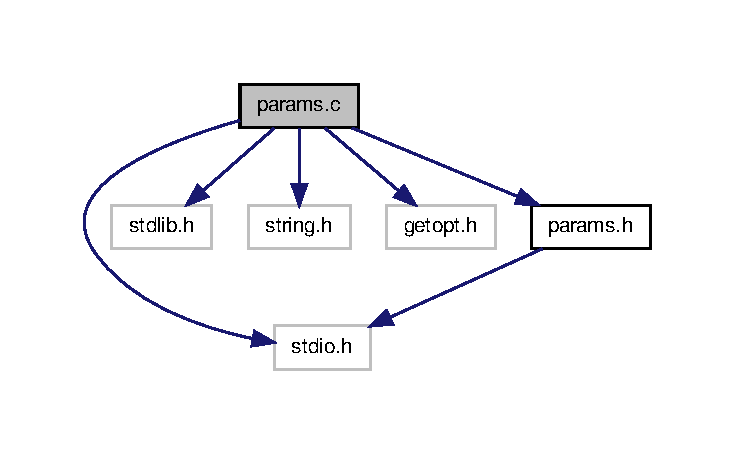
\includegraphics[width=352pt]{d7/d4b/params_8c__incl}
\end{center}
\end{figure}
\subsection*{Data Structures}
\begin{DoxyCompactItemize}
\item 
struct {\bf line\_\-list}
\end{DoxyCompactItemize}
\subsection*{Defines}
\begin{DoxyCompactItemize}
\item 
\#define {\bf FIX\_\-UNUSED}(X)~(void) (X)
\item 
\#define {\bf CONFIG\_\-FILE\_\-LINE\_\-SIZE}~2048
\item 
\#define {\bf ADDITIONAL\_\-ERROR}~\char`\"{} in configuration file \char`\"{}
\item 
\#define {\bf CONFIG\_\-FILE\_\-LINE\_\-BUFFER\_\-SIZE}~(CONFIG\_\-FILE\_\-LINE\_\-SIZE+3)
\end{DoxyCompactItemize}
\subsection*{Enumerations}
\begin{DoxyCompactItemize}
\item 
enum {\bf cmdline\_\-parser\_\-arg\_\-type} \{ {\bf ARG\_\-NO}, 
{\bf ARG\_\-STRING}
 \}
\end{DoxyCompactItemize}
\subsection*{Functions}
\begin{DoxyCompactItemize}
\item 
void {\bf cmdline\_\-parser\_\-print\_\-version} (void)
\item 
void {\bf cmdline\_\-parser\_\-print\_\-help} (void)
\item 
void {\bf cmdline\_\-parser\_\-init} (struct {\bf gengetopt\_\-args\_\-info} $\ast$args\_\-info)
\item 
void {\bf cmdline\_\-parser\_\-params\_\-init} (struct {\bf cmdline\_\-parser\_\-params} $\ast$params)
\item 
struct {\bf cmdline\_\-parser\_\-params} $\ast$ {\bf cmdline\_\-parser\_\-params\_\-create} (void)
\item 
int {\bf cmdline\_\-parser\_\-dump} (FILE $\ast$outfile, struct {\bf gengetopt\_\-args\_\-info} $\ast$args\_\-info)
\item 
int {\bf cmdline\_\-parser\_\-file\_\-save} (const char $\ast$filename, struct {\bf gengetopt\_\-args\_\-info} $\ast$args\_\-info)
\item 
void {\bf cmdline\_\-parser\_\-free} (struct {\bf gengetopt\_\-args\_\-info} $\ast$args\_\-info)
\item 
int {\bf cmdline\_\-parser} (int argc, char $\ast$$\ast$argv, struct {\bf gengetopt\_\-args\_\-info} $\ast$args\_\-info)
\item 
int {\bf cmdline\_\-parser\_\-ext} (int argc, char $\ast$$\ast$argv, struct {\bf gengetopt\_\-args\_\-info} $\ast$args\_\-info, struct {\bf cmdline\_\-parser\_\-params} $\ast$params)
\item 
int {\bf cmdline\_\-parser2} (int argc, char $\ast$$\ast$argv, struct {\bf gengetopt\_\-args\_\-info} $\ast$args\_\-info, int override, int initialize, int check\_\-required)
\item 
int {\bf cmdline\_\-parser\_\-required} (struct {\bf gengetopt\_\-args\_\-info} $\ast$args\_\-info, const char $\ast$prog\_\-name)
\item 
int {\bf cmdline\_\-parser\_\-configfile} (const char $\ast$filename, struct {\bf gengetopt\_\-args\_\-info} $\ast$args\_\-info, int override, int initialize, int check\_\-required)
\item 
int {\bf cmdline\_\-parser\_\-config\_\-file} (const char $\ast$filename, struct {\bf gengetopt\_\-args\_\-info} $\ast$args\_\-info, struct {\bf cmdline\_\-parser\_\-params} $\ast$params)
\end{DoxyCompactItemize}
\subsection*{Variables}
\begin{DoxyCompactItemize}
\item 
const char $\ast$ {\bf gengetopt\_\-args\_\-info\_\-purpose} = \char`\"{}O programa é responsavel por codificar uma imagem usando CUDA\char`\"{}
\begin{DoxyCompactList}\small\item\em the purpose string of the program \end{DoxyCompactList}\item 
const char $\ast$ {\bf gengetopt\_\-args\_\-info\_\-usage} = \char`\"{}Usage: Encoder [OPTIONS]... [FILES]...\char`\"{}
\begin{DoxyCompactList}\small\item\em the usage string of the program \end{DoxyCompactList}\item 
const char $\ast$ {\bf gengetopt\_\-args\_\-info\_\-description} = \char`\"{}\char`\"{}
\item 
const char $\ast$ {\bf gengetopt\_\-args\_\-info\_\-help} [$\,$]
\begin{DoxyCompactList}\small\item\em all the lines making the help output \end{DoxyCompactList}\end{DoxyCompactItemize}


\subsection{Define Documentation}
\index{params.c@{params.c}!ADDITIONAL\_\-ERROR@{ADDITIONAL\_\-ERROR}}
\index{ADDITIONAL\_\-ERROR@{ADDITIONAL\_\-ERROR}!params.c@{params.c}}
\subsubsection[{ADDITIONAL\_\-ERROR}]{\setlength{\rightskip}{0pt plus 5cm}\#define ADDITIONAL\_\-ERROR~\char`\"{} in configuration file \char`\"{}}\label{da/de3/params_8c_ab8f5eb4c8f558f0cce031c6aa30b3441}
\index{params.c@{params.c}!CONFIG\_\-FILE\_\-LINE\_\-BUFFER\_\-SIZE@{CONFIG\_\-FILE\_\-LINE\_\-BUFFER\_\-SIZE}}
\index{CONFIG\_\-FILE\_\-LINE\_\-BUFFER\_\-SIZE@{CONFIG\_\-FILE\_\-LINE\_\-BUFFER\_\-SIZE}!params.c@{params.c}}
\subsubsection[{CONFIG\_\-FILE\_\-LINE\_\-BUFFER\_\-SIZE}]{\setlength{\rightskip}{0pt plus 5cm}\#define CONFIG\_\-FILE\_\-LINE\_\-BUFFER\_\-SIZE~(CONFIG\_\-FILE\_\-LINE\_\-SIZE+3)}\label{da/de3/params_8c_a3b209de56f1b67fb95662576aa5a0ab9}
\index{params.c@{params.c}!CONFIG\_\-FILE\_\-LINE\_\-SIZE@{CONFIG\_\-FILE\_\-LINE\_\-SIZE}}
\index{CONFIG\_\-FILE\_\-LINE\_\-SIZE@{CONFIG\_\-FILE\_\-LINE\_\-SIZE}!params.c@{params.c}}
\subsubsection[{CONFIG\_\-FILE\_\-LINE\_\-SIZE}]{\setlength{\rightskip}{0pt plus 5cm}\#define CONFIG\_\-FILE\_\-LINE\_\-SIZE~2048}\label{da/de3/params_8c_a6f5db5e4f74ca5ffbdda87292ac649ad}
\index{params.c@{params.c}!FIX\_\-UNUSED@{FIX\_\-UNUSED}}
\index{FIX\_\-UNUSED@{FIX\_\-UNUSED}!params.c@{params.c}}
\subsubsection[{FIX\_\-UNUSED}]{\setlength{\rightskip}{0pt plus 5cm}\#define FIX\_\-UNUSED(
\begin{DoxyParamCaption}
\item[{}]{X}
\end{DoxyParamCaption}
)~(void) (X)}\label{da/de3/params_8c_a8db449d7b07c45ef8a58716e09eba04e}


\subsection{Enumeration Type Documentation}
\index{params.c@{params.c}!cmdline\_\-parser\_\-arg\_\-type@{cmdline\_\-parser\_\-arg\_\-type}}
\index{cmdline\_\-parser\_\-arg\_\-type@{cmdline\_\-parser\_\-arg\_\-type}!params.c@{params.c}}
\subsubsection[{cmdline\_\-parser\_\-arg\_\-type}]{\setlength{\rightskip}{0pt plus 5cm}enum {\bf cmdline\_\-parser\_\-arg\_\-type}}\label{da/de3/params_8c_a88e31a859f36efa57ad64e6ae13332a1}
\begin{Desc}
\item[Enumerator: ]\par
\begin{description}
\index{ARG\_\-NO@{ARG\_\-NO}!params.c@{params.c}}\index{params.c@{params.c}!ARG\_\-NO@{ARG\_\-NO}}\item[{\em 
ARG\_\-NO\label{da/de3/params_8c_a88e31a859f36efa57ad64e6ae13332a1a67dd250fb3e23862523b667407868ada}
}]\index{ARG\_\-STRING@{ARG\_\-STRING}!params.c@{params.c}}\index{params.c@{params.c}!ARG\_\-STRING@{ARG\_\-STRING}}\item[{\em 
ARG\_\-STRING\label{da/de3/params_8c_a88e31a859f36efa57ad64e6ae13332a1a1e0904ee5e3baf2aa4070ab0718a3afa}
}]\end{description}
\end{Desc}



\subsection{Function Documentation}
\index{params.c@{params.c}!cmdline\_\-parser@{cmdline\_\-parser}}
\index{cmdline\_\-parser@{cmdline\_\-parser}!params.c@{params.c}}
\subsubsection[{cmdline\_\-parser}]{\setlength{\rightskip}{0pt plus 5cm}int cmdline\_\-parser (
\begin{DoxyParamCaption}
\item[{int}]{argc, }
\item[{char $\ast$$\ast$}]{argv, }
\item[{struct {\bf gengetopt\_\-args\_\-info} $\ast$}]{args\_\-info}
\end{DoxyParamCaption}
)}\label{da/de3/params_8c_a3c3df73307452c51fee0a34640d92196}
The command line parser 
\begin{DoxyParams}{Parameters}
{\em argc} & the number of command line options \\
\hline
{\em argv} & the command line options \\
\hline
{\em args\_\-info} & the structure where option information will be stored \\
\hline
\end{DoxyParams}
\begin{DoxyReturn}{Returns}
0 if everything went fine, NON 0 if an error took place 
\end{DoxyReturn}
\index{params.c@{params.c}!cmdline\_\-parser2@{cmdline\_\-parser2}}
\index{cmdline\_\-parser2@{cmdline\_\-parser2}!params.c@{params.c}}
\subsubsection[{cmdline\_\-parser2}]{\setlength{\rightskip}{0pt plus 5cm}int cmdline\_\-parser2 (
\begin{DoxyParamCaption}
\item[{int}]{argc, }
\item[{char $\ast$$\ast$}]{argv, }
\item[{struct {\bf gengetopt\_\-args\_\-info} $\ast$}]{args\_\-info, }
\item[{int}]{override, }
\item[{int}]{initialize, }
\item[{int}]{check\_\-required}
\end{DoxyParamCaption}
)}\label{da/de3/params_8c_a78a0cd581698415a62f68214603b1a30}
The command line parser (version with additional parameters -\/ deprecated) 
\begin{DoxyParams}{Parameters}
{\em argc} & the number of command line options \\
\hline
{\em argv} & the command line options \\
\hline
{\em args\_\-info} & the structure where option information will be stored \\
\hline
{\em override} & whether to override possibly already present options \\
\hline
{\em initialize} & whether to initialize the option structure my\_\-args\_\-info \\
\hline
{\em check\_\-required} & whether to check that all required options were provided \\
\hline
\end{DoxyParams}
\begin{DoxyReturn}{Returns}
0 if everything went fine, NON 0 if an error took place 
\end{DoxyReturn}
\begin{Desc}
\item[{\bf Deprecated}]use \doxyref{cmdline\_\-parser\_\-ext()}{p.}{da/de3/params_8c_ac7bb5d76f3f56d1c0b3b531f11ac6f07} instead \end{Desc}
\index{params.c@{params.c}!cmdline\_\-parser\_\-config\_\-file@{cmdline\_\-parser\_\-config\_\-file}}
\index{cmdline\_\-parser\_\-config\_\-file@{cmdline\_\-parser\_\-config\_\-file}!params.c@{params.c}}
\subsubsection[{cmdline\_\-parser\_\-config\_\-file}]{\setlength{\rightskip}{0pt plus 5cm}int cmdline\_\-parser\_\-config\_\-file (
\begin{DoxyParamCaption}
\item[{const char $\ast$}]{filename, }
\item[{struct {\bf gengetopt\_\-args\_\-info} $\ast$}]{args\_\-info, }
\item[{struct {\bf cmdline\_\-parser\_\-params} $\ast$}]{params}
\end{DoxyParamCaption}
)}\label{da/de3/params_8c_adc206332aa07c44a515d8bc11b280686}
The config file parser 
\begin{DoxyParams}{Parameters}
{\em filename} & the name of the config file \\
\hline
{\em args\_\-info} & the structure where option information will be stored \\
\hline
{\em params} & additional parameters for the parser \\
\hline
\end{DoxyParams}
\begin{DoxyReturn}{Returns}
0 if everything went fine, NON 0 if an error took place 
\end{DoxyReturn}
\index{params.c@{params.c}!cmdline\_\-parser\_\-configfile@{cmdline\_\-parser\_\-configfile}}
\index{cmdline\_\-parser\_\-configfile@{cmdline\_\-parser\_\-configfile}!params.c@{params.c}}
\subsubsection[{cmdline\_\-parser\_\-configfile}]{\setlength{\rightskip}{0pt plus 5cm}int cmdline\_\-parser\_\-configfile (
\begin{DoxyParamCaption}
\item[{const char $\ast$}]{filename, }
\item[{struct {\bf gengetopt\_\-args\_\-info} $\ast$}]{args\_\-info, }
\item[{int}]{override, }
\item[{int}]{initialize, }
\item[{int}]{check\_\-required}
\end{DoxyParamCaption}
)}\label{da/de3/params_8c_affdc7d48ef44983e319430c0888cb310}
The config file parser (deprecated version) 
\begin{DoxyParams}{Parameters}
{\em filename} & the name of the config file \\
\hline
{\em args\_\-info} & the structure where option information will be stored \\
\hline
{\em override} & whether to override possibly already present options \\
\hline
{\em initialize} & whether to initialize the option structure my\_\-args\_\-info \\
\hline
{\em check\_\-required} & whether to check that all required options were provided \\
\hline
\end{DoxyParams}
\begin{DoxyReturn}{Returns}
0 if everything went fine, NON 0 if an error took place 
\end{DoxyReturn}
\begin{Desc}
\item[{\bf Deprecated}]use \doxyref{cmdline\_\-parser\_\-config\_\-file()}{p.}{da/de3/params_8c_adc206332aa07c44a515d8bc11b280686} instead \end{Desc}
\index{params.c@{params.c}!cmdline\_\-parser\_\-dump@{cmdline\_\-parser\_\-dump}}
\index{cmdline\_\-parser\_\-dump@{cmdline\_\-parser\_\-dump}!params.c@{params.c}}
\subsubsection[{cmdline\_\-parser\_\-dump}]{\setlength{\rightskip}{0pt plus 5cm}int cmdline\_\-parser\_\-dump (
\begin{DoxyParamCaption}
\item[{FILE $\ast$}]{outfile, }
\item[{struct {\bf gengetopt\_\-args\_\-info} $\ast$}]{args\_\-info}
\end{DoxyParamCaption}
)}\label{da/de3/params_8c_a1f73418092a6e6eb3706aa0de2785e11}
Save the contents of the option struct into an already open FILE stream. 
\begin{DoxyParams}{Parameters}
{\em outfile} & the stream where to dump options \\
\hline
{\em args\_\-info} & the option struct to dump \\
\hline
\end{DoxyParams}
\begin{DoxyReturn}{Returns}
0 if everything went fine, NON 0 if an error took place 
\end{DoxyReturn}
\index{params.c@{params.c}!cmdline\_\-parser\_\-ext@{cmdline\_\-parser\_\-ext}}
\index{cmdline\_\-parser\_\-ext@{cmdline\_\-parser\_\-ext}!params.c@{params.c}}
\subsubsection[{cmdline\_\-parser\_\-ext}]{\setlength{\rightskip}{0pt plus 5cm}int cmdline\_\-parser\_\-ext (
\begin{DoxyParamCaption}
\item[{int}]{argc, }
\item[{char $\ast$$\ast$}]{argv, }
\item[{struct {\bf gengetopt\_\-args\_\-info} $\ast$}]{args\_\-info, }
\item[{struct {\bf cmdline\_\-parser\_\-params} $\ast$}]{params}
\end{DoxyParamCaption}
)}\label{da/de3/params_8c_ac7bb5d76f3f56d1c0b3b531f11ac6f07}
The command line parser (version with additional parameters) 
\begin{DoxyParams}{Parameters}
{\em argc} & the number of command line options \\
\hline
{\em argv} & the command line options \\
\hline
{\em args\_\-info} & the structure where option information will be stored \\
\hline
{\em params} & additional parameters for the parser \\
\hline
\end{DoxyParams}
\begin{DoxyReturn}{Returns}
0 if everything went fine, NON 0 if an error took place 
\end{DoxyReturn}
\index{params.c@{params.c}!cmdline\_\-parser\_\-file\_\-save@{cmdline\_\-parser\_\-file\_\-save}}
\index{cmdline\_\-parser\_\-file\_\-save@{cmdline\_\-parser\_\-file\_\-save}!params.c@{params.c}}
\subsubsection[{cmdline\_\-parser\_\-file\_\-save}]{\setlength{\rightskip}{0pt plus 5cm}int cmdline\_\-parser\_\-file\_\-save (
\begin{DoxyParamCaption}
\item[{const char $\ast$}]{filename, }
\item[{struct {\bf gengetopt\_\-args\_\-info} $\ast$}]{args\_\-info}
\end{DoxyParamCaption}
)}\label{da/de3/params_8c_a5f3e9412f88f1058a31ac28ad2ea2818}
Save the contents of the option struct into a (text) file. This file can be read by the config file parser (if generated by gengetopt) 
\begin{DoxyParams}{Parameters}
{\em filename} & the file where to save \\
\hline
{\em args\_\-info} & the option struct to save \\
\hline
\end{DoxyParams}
\begin{DoxyReturn}{Returns}
0 if everything went fine, NON 0 if an error took place 
\end{DoxyReturn}
\index{params.c@{params.c}!cmdline\_\-parser\_\-free@{cmdline\_\-parser\_\-free}}
\index{cmdline\_\-parser\_\-free@{cmdline\_\-parser\_\-free}!params.c@{params.c}}
\subsubsection[{cmdline\_\-parser\_\-free}]{\setlength{\rightskip}{0pt plus 5cm}void cmdline\_\-parser\_\-free (
\begin{DoxyParamCaption}
\item[{struct {\bf gengetopt\_\-args\_\-info} $\ast$}]{args\_\-info}
\end{DoxyParamCaption}
)}\label{da/de3/params_8c_af1b97c4e92b88f736e350b3902266ba4}
Deallocates the string fields of the \doxyref{gengetopt\_\-args\_\-info}{p.}{da/dad/structgengetopt__args__info} structure (but does not deallocate the structure itself) 
\begin{DoxyParams}{Parameters}
{\em args\_\-info} & the structure to deallocate \\
\hline
\end{DoxyParams}
\index{params.c@{params.c}!cmdline\_\-parser\_\-init@{cmdline\_\-parser\_\-init}}
\index{cmdline\_\-parser\_\-init@{cmdline\_\-parser\_\-init}!params.c@{params.c}}
\subsubsection[{cmdline\_\-parser\_\-init}]{\setlength{\rightskip}{0pt plus 5cm}void cmdline\_\-parser\_\-init (
\begin{DoxyParamCaption}
\item[{struct {\bf gengetopt\_\-args\_\-info} $\ast$}]{args\_\-info}
\end{DoxyParamCaption}
)}\label{da/de3/params_8c_aca62b50d03d0d082968eeb1940f98650}
Initializes the passed \doxyref{gengetopt\_\-args\_\-info}{p.}{da/dad/structgengetopt__args__info} structure's fields (also set default values for options that have a default) 
\begin{DoxyParams}{Parameters}
{\em args\_\-info} & the structure to initialize \\
\hline
\end{DoxyParams}
\index{params.c@{params.c}!cmdline\_\-parser\_\-params\_\-create@{cmdline\_\-parser\_\-params\_\-create}}
\index{cmdline\_\-parser\_\-params\_\-create@{cmdline\_\-parser\_\-params\_\-create}!params.c@{params.c}}
\subsubsection[{cmdline\_\-parser\_\-params\_\-create}]{\setlength{\rightskip}{0pt plus 5cm}struct {\bf cmdline\_\-parser\_\-params}$\ast$ cmdline\_\-parser\_\-params\_\-create (
\begin{DoxyParamCaption}
\item[{void}]{}
\end{DoxyParamCaption}
)\hspace{0.3cm}{\ttfamily  [read]}}\label{da/de3/params_8c_afd778af110fe0ee1ea5eac7aa9939d92}
Allocates dynamically a \doxyref{cmdline\_\-parser\_\-params}{p.}{db/d02/structcmdline__parser__params} structure and initializes all its fields to their default values \begin{DoxyReturn}{Returns}
the created and initialized \doxyref{cmdline\_\-parser\_\-params}{p.}{db/d02/structcmdline__parser__params} structure 
\end{DoxyReturn}
\index{params.c@{params.c}!cmdline\_\-parser\_\-params\_\-init@{cmdline\_\-parser\_\-params\_\-init}}
\index{cmdline\_\-parser\_\-params\_\-init@{cmdline\_\-parser\_\-params\_\-init}!params.c@{params.c}}
\subsubsection[{cmdline\_\-parser\_\-params\_\-init}]{\setlength{\rightskip}{0pt plus 5cm}void cmdline\_\-parser\_\-params\_\-init (
\begin{DoxyParamCaption}
\item[{struct {\bf cmdline\_\-parser\_\-params} $\ast$}]{params}
\end{DoxyParamCaption}
)}\label{da/de3/params_8c_af72b814611cffc706b2135ccdfe7e997}
Initializes all the fields a \doxyref{cmdline\_\-parser\_\-params}{p.}{db/d02/structcmdline__parser__params} structure to their default values 
\begin{DoxyParams}{Parameters}
{\em params} & the structure to initialize \\
\hline
\end{DoxyParams}
\index{params.c@{params.c}!cmdline\_\-parser\_\-print\_\-help@{cmdline\_\-parser\_\-print\_\-help}}
\index{cmdline\_\-parser\_\-print\_\-help@{cmdline\_\-parser\_\-print\_\-help}!params.c@{params.c}}
\subsubsection[{cmdline\_\-parser\_\-print\_\-help}]{\setlength{\rightskip}{0pt plus 5cm}void cmdline\_\-parser\_\-print\_\-help (
\begin{DoxyParamCaption}
\item[{void}]{}
\end{DoxyParamCaption}
)}\label{da/de3/params_8c_ad4f7db2fa4002379eb30e5206f3b7492}
Print the help \index{params.c@{params.c}!cmdline\_\-parser\_\-print\_\-version@{cmdline\_\-parser\_\-print\_\-version}}
\index{cmdline\_\-parser\_\-print\_\-version@{cmdline\_\-parser\_\-print\_\-version}!params.c@{params.c}}
\subsubsection[{cmdline\_\-parser\_\-print\_\-version}]{\setlength{\rightskip}{0pt plus 5cm}void cmdline\_\-parser\_\-print\_\-version (
\begin{DoxyParamCaption}
\item[{void}]{}
\end{DoxyParamCaption}
)}\label{da/de3/params_8c_a96f27bf35ce0ab8eea7a1f6e6b59a5e2}
Print the version \index{params.c@{params.c}!cmdline\_\-parser\_\-required@{cmdline\_\-parser\_\-required}}
\index{cmdline\_\-parser\_\-required@{cmdline\_\-parser\_\-required}!params.c@{params.c}}
\subsubsection[{cmdline\_\-parser\_\-required}]{\setlength{\rightskip}{0pt plus 5cm}int cmdline\_\-parser\_\-required (
\begin{DoxyParamCaption}
\item[{struct {\bf gengetopt\_\-args\_\-info} $\ast$}]{args\_\-info, }
\item[{const char $\ast$}]{prog\_\-name}
\end{DoxyParamCaption}
)}\label{da/de3/params_8c_a83651e5be280d60aed58fdb72456a030}
Checks that all the required options were specified 
\begin{DoxyParams}{Parameters}
{\em args\_\-info} & the structure to check \\
\hline
{\em prog\_\-name} & the name of the program that will be used to print possible errors \\
\hline
\end{DoxyParams}
\begin{DoxyReturn}{Returns}

\end{DoxyReturn}


\subsection{Variable Documentation}
\index{params.c@{params.c}!gengetopt\_\-args\_\-info\_\-description@{gengetopt\_\-args\_\-info\_\-description}}
\index{gengetopt\_\-args\_\-info\_\-description@{gengetopt\_\-args\_\-info\_\-description}!params.c@{params.c}}
\subsubsection[{gengetopt\_\-args\_\-info\_\-description}]{\setlength{\rightskip}{0pt plus 5cm}const char$\ast$ {\bf gengetopt\_\-args\_\-info\_\-description} = \char`\"{}\char`\"{}}\label{da/de3/params_8c_accad6107ca685f6eba555f6ce63d355d}
\index{params.c@{params.c}!gengetopt\_\-args\_\-info\_\-help@{gengetopt\_\-args\_\-info\_\-help}}
\index{gengetopt\_\-args\_\-info\_\-help@{gengetopt\_\-args\_\-info\_\-help}!params.c@{params.c}}
\subsubsection[{gengetopt\_\-args\_\-info\_\-help}]{\setlength{\rightskip}{0pt plus 5cm}const char$\ast$ {\bf gengetopt\_\-args\_\-info\_\-help}[$\,$]}\label{da/de3/params_8c_a6af7a6b7fb37c0abaa916ee1cfa0a41f}
{\bfseries Initial value:}
\begin{DoxyCode}
 {
  "  -h, --help               Print help and exit",
  "  -V, --version            Print version and exit",
  "  -i, --imagem=STRING      nome da imagem PGM a ser codificada",
  "  -d, --dicionario=STRING  nome do dicionario de codificação",
  "  -o, --ficheiro=STRING    nome do ficheiro de saída (ficheiro codificado)",
    0
}
\end{DoxyCode}


all the lines making the help output 

\index{params.c@{params.c}!gengetopt\_\-args\_\-info\_\-purpose@{gengetopt\_\-args\_\-info\_\-purpose}}
\index{gengetopt\_\-args\_\-info\_\-purpose@{gengetopt\_\-args\_\-info\_\-purpose}!params.c@{params.c}}
\subsubsection[{gengetopt\_\-args\_\-info\_\-purpose}]{\setlength{\rightskip}{0pt plus 5cm}const char$\ast$ {\bf gengetopt\_\-args\_\-info\_\-purpose} = \char`\"{}O programa é responsavel por codificar uma imagem usando CUDA\char`\"{}}\label{da/de3/params_8c_a610c3307abce5a8fd304b86b018ae60b}


the purpose string of the program 

\index{params.c@{params.c}!gengetopt\_\-args\_\-info\_\-usage@{gengetopt\_\-args\_\-info\_\-usage}}
\index{gengetopt\_\-args\_\-info\_\-usage@{gengetopt\_\-args\_\-info\_\-usage}!params.c@{params.c}}
\subsubsection[{gengetopt\_\-args\_\-info\_\-usage}]{\setlength{\rightskip}{0pt plus 5cm}const char$\ast$ {\bf gengetopt\_\-args\_\-info\_\-usage} = \char`\"{}Usage: Encoder [OPTIONS]... [FILES]...\char`\"{}}\label{da/de3/params_8c_a9f397a306f363bfdebb611e86acf36d5}


the usage string of the program 


\section{params.h File Reference}
\label{da/d33/params_8h}\index{params.h@{params.h}}


The header file for the command line option parser generated by GNU Gengetopt version 2.22.4 {\tt http://www.gnu.org/software/gengetopt.} DO NOT modify this file, since it can be overwritten.  


{\ttfamily \#include $<$stdio.h$>$}\par
Include dependency graph for params.h:\nopagebreak
\begin{figure}[H]
\begin{center}
\leavevmode
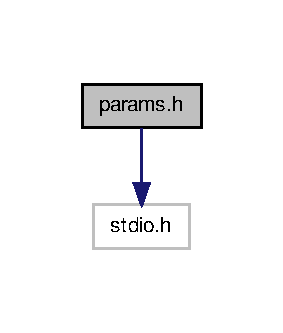
\includegraphics[width=136pt]{dc/d97/params_8h__incl}
\end{center}
\end{figure}
This graph shows which files directly or indirectly include this file:\nopagebreak
\begin{figure}[H]
\begin{center}
\leavevmode
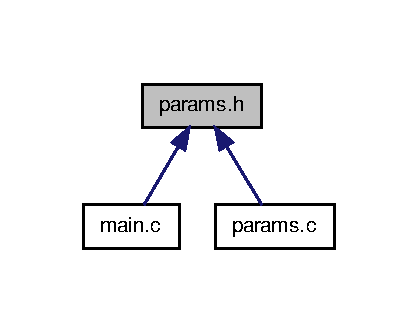
\includegraphics[width=200pt]{d8/d6f/params_8h__dep__incl}
\end{center}
\end{figure}
\subsection*{Data Structures}
\begin{DoxyCompactItemize}
\item 
struct {\bf gengetopt\_\-args\_\-info}
\begin{DoxyCompactList}\small\item\em Where the command line options are stored. \end{DoxyCompactList}\item 
struct {\bf cmdline\_\-parser\_\-params}
\begin{DoxyCompactList}\small\item\em The additional parameters to pass to parser functions. \end{DoxyCompactList}\end{DoxyCompactItemize}
\subsection*{Defines}
\begin{DoxyCompactItemize}
\item 
\#define {\bf CMDLINE\_\-PARSER\_\-PACKAGE}~\char`\"{}Encoder\char`\"{}
\begin{DoxyCompactList}\small\item\em the program name (used for printing errors) \end{DoxyCompactList}\item 
\#define {\bf CMDLINE\_\-PARSER\_\-PACKAGE\_\-NAME}~\char`\"{}Encoder\char`\"{}
\begin{DoxyCompactList}\small\item\em the complete program name (used for help and version) \end{DoxyCompactList}\item 
\#define {\bf CMDLINE\_\-PARSER\_\-VERSION}~\char`\"{}v1.0.0\char`\"{}
\begin{DoxyCompactList}\small\item\em the program version \end{DoxyCompactList}\end{DoxyCompactItemize}
\subsection*{Functions}
\begin{DoxyCompactItemize}
\item 
int {\bf cmdline\_\-parser} (int argc, char $\ast$$\ast$argv, struct {\bf gengetopt\_\-args\_\-info} $\ast$args\_\-info)
\item 
int {\bf cmdline\_\-parser2} (int argc, char $\ast$$\ast$argv, struct {\bf gengetopt\_\-args\_\-info} $\ast$args\_\-info, int override, int initialize, int check\_\-required)
\item 
int {\bf cmdline\_\-parser\_\-ext} (int argc, char $\ast$$\ast$argv, struct {\bf gengetopt\_\-args\_\-info} $\ast$args\_\-info, struct {\bf cmdline\_\-parser\_\-params} $\ast$params)
\item 
int {\bf cmdline\_\-parser\_\-dump} (FILE $\ast$outfile, struct {\bf gengetopt\_\-args\_\-info} $\ast$args\_\-info)
\item 
int {\bf cmdline\_\-parser\_\-file\_\-save} (const char $\ast$filename, struct {\bf gengetopt\_\-args\_\-info} $\ast$args\_\-info)
\item 
void {\bf cmdline\_\-parser\_\-print\_\-help} (void)
\item 
void {\bf cmdline\_\-parser\_\-print\_\-version} (void)
\item 
void {\bf cmdline\_\-parser\_\-params\_\-init} (struct {\bf cmdline\_\-parser\_\-params} $\ast$params)
\item 
struct {\bf cmdline\_\-parser\_\-params} $\ast$ {\bf cmdline\_\-parser\_\-params\_\-create} (void)
\item 
void {\bf cmdline\_\-parser\_\-init} (struct {\bf gengetopt\_\-args\_\-info} $\ast$args\_\-info)
\item 
void {\bf cmdline\_\-parser\_\-free} (struct {\bf gengetopt\_\-args\_\-info} $\ast$args\_\-info)
\item 
int {\bf cmdline\_\-parser\_\-configfile} (const char $\ast$filename, struct {\bf gengetopt\_\-args\_\-info} $\ast$args\_\-info, int override, int initialize, int check\_\-required)
\item 
int {\bf cmdline\_\-parser\_\-config\_\-file} (const char $\ast$filename, struct {\bf gengetopt\_\-args\_\-info} $\ast$args\_\-info, struct {\bf cmdline\_\-parser\_\-params} $\ast$params)
\item 
int {\bf cmdline\_\-parser\_\-required} (struct {\bf gengetopt\_\-args\_\-info} $\ast$args\_\-info, const char $\ast$prog\_\-name)
\end{DoxyCompactItemize}
\subsection*{Variables}
\begin{DoxyCompactItemize}
\item 
const char $\ast$ {\bf gengetopt\_\-args\_\-info\_\-purpose}
\begin{DoxyCompactList}\small\item\em the purpose string of the program \end{DoxyCompactList}\item 
const char $\ast$ {\bf gengetopt\_\-args\_\-info\_\-usage}
\begin{DoxyCompactList}\small\item\em the usage string of the program \end{DoxyCompactList}\item 
const char $\ast$ {\bf gengetopt\_\-args\_\-info\_\-help} [$\,$]
\begin{DoxyCompactList}\small\item\em all the lines making the help output \end{DoxyCompactList}\end{DoxyCompactItemize}


\subsection{Detailed Description}
The header file for the command line option parser generated by GNU Gengetopt version 2.22.4 {\tt http://www.gnu.org/software/gengetopt.} DO NOT modify this file, since it can be overwritten. \begin{DoxyAuthor}{Author}
GNU Gengetopt by Lorenzo Bettini 
\end{DoxyAuthor}


\subsection{Define Documentation}
\index{params.h@{params.h}!CMDLINE\_\-PARSER\_\-PACKAGE@{CMDLINE\_\-PARSER\_\-PACKAGE}}
\index{CMDLINE\_\-PARSER\_\-PACKAGE@{CMDLINE\_\-PARSER\_\-PACKAGE}!params.h@{params.h}}
\subsubsection[{CMDLINE\_\-PARSER\_\-PACKAGE}]{\setlength{\rightskip}{0pt plus 5cm}\#define CMDLINE\_\-PARSER\_\-PACKAGE~\char`\"{}Encoder\char`\"{}}\label{da/d33/params_8h_aeb847973552c32bcbe5f14973a0a8a32}


the program name (used for printing errors) 

\index{params.h@{params.h}!CMDLINE\_\-PARSER\_\-PACKAGE\_\-NAME@{CMDLINE\_\-PARSER\_\-PACKAGE\_\-NAME}}
\index{CMDLINE\_\-PARSER\_\-PACKAGE\_\-NAME@{CMDLINE\_\-PARSER\_\-PACKAGE\_\-NAME}!params.h@{params.h}}
\subsubsection[{CMDLINE\_\-PARSER\_\-PACKAGE\_\-NAME}]{\setlength{\rightskip}{0pt plus 5cm}\#define CMDLINE\_\-PARSER\_\-PACKAGE\_\-NAME~\char`\"{}Encoder\char`\"{}}\label{da/d33/params_8h_ae2f94765d0d8758ddf6b326a4806d6ff}


the complete program name (used for help and version) 

\index{params.h@{params.h}!CMDLINE\_\-PARSER\_\-VERSION@{CMDLINE\_\-PARSER\_\-VERSION}}
\index{CMDLINE\_\-PARSER\_\-VERSION@{CMDLINE\_\-PARSER\_\-VERSION}!params.h@{params.h}}
\subsubsection[{CMDLINE\_\-PARSER\_\-VERSION}]{\setlength{\rightskip}{0pt plus 5cm}\#define CMDLINE\_\-PARSER\_\-VERSION~\char`\"{}v1.0.0\char`\"{}}\label{da/d33/params_8h_a1eeca7dc254bf6867ba9635f45771471}


the program version 



\subsection{Function Documentation}
\index{params.h@{params.h}!cmdline\_\-parser@{cmdline\_\-parser}}
\index{cmdline\_\-parser@{cmdline\_\-parser}!params.h@{params.h}}
\subsubsection[{cmdline\_\-parser}]{\setlength{\rightskip}{0pt plus 5cm}int cmdline\_\-parser (
\begin{DoxyParamCaption}
\item[{int}]{argc, }
\item[{char $\ast$$\ast$}]{argv, }
\item[{struct {\bf gengetopt\_\-args\_\-info} $\ast$}]{args\_\-info}
\end{DoxyParamCaption}
)}\label{da/d33/params_8h_a3c3df73307452c51fee0a34640d92196}
The command line parser 
\begin{DoxyParams}{Parameters}
{\em argc} & the number of command line options \\
\hline
{\em argv} & the command line options \\
\hline
{\em args\_\-info} & the structure where option information will be stored \\
\hline
\end{DoxyParams}
\begin{DoxyReturn}{Returns}
0 if everything went fine, NON 0 if an error took place 
\end{DoxyReturn}
\index{params.h@{params.h}!cmdline\_\-parser2@{cmdline\_\-parser2}}
\index{cmdline\_\-parser2@{cmdline\_\-parser2}!params.h@{params.h}}
\subsubsection[{cmdline\_\-parser2}]{\setlength{\rightskip}{0pt plus 5cm}int cmdline\_\-parser2 (
\begin{DoxyParamCaption}
\item[{int}]{argc, }
\item[{char $\ast$$\ast$}]{argv, }
\item[{struct {\bf gengetopt\_\-args\_\-info} $\ast$}]{args\_\-info, }
\item[{int}]{override, }
\item[{int}]{initialize, }
\item[{int}]{check\_\-required}
\end{DoxyParamCaption}
)}\label{da/d33/params_8h_a78a0cd581698415a62f68214603b1a30}
The command line parser (version with additional parameters -\/ deprecated) 
\begin{DoxyParams}{Parameters}
{\em argc} & the number of command line options \\
\hline
{\em argv} & the command line options \\
\hline
{\em args\_\-info} & the structure where option information will be stored \\
\hline
{\em override} & whether to override possibly already present options \\
\hline
{\em initialize} & whether to initialize the option structure my\_\-args\_\-info \\
\hline
{\em check\_\-required} & whether to check that all required options were provided \\
\hline
\end{DoxyParams}
\begin{DoxyReturn}{Returns}
0 if everything went fine, NON 0 if an error took place 
\end{DoxyReturn}
\begin{Desc}
\item[{\bf Deprecated}]use \doxyref{cmdline\_\-parser\_\-ext()}{p.}{da/de3/params_8c_ac7bb5d76f3f56d1c0b3b531f11ac6f07} instead \end{Desc}
\index{params.h@{params.h}!cmdline\_\-parser\_\-config\_\-file@{cmdline\_\-parser\_\-config\_\-file}}
\index{cmdline\_\-parser\_\-config\_\-file@{cmdline\_\-parser\_\-config\_\-file}!params.h@{params.h}}
\subsubsection[{cmdline\_\-parser\_\-config\_\-file}]{\setlength{\rightskip}{0pt plus 5cm}int cmdline\_\-parser\_\-config\_\-file (
\begin{DoxyParamCaption}
\item[{const char $\ast$}]{filename, }
\item[{struct {\bf gengetopt\_\-args\_\-info} $\ast$}]{args\_\-info, }
\item[{struct {\bf cmdline\_\-parser\_\-params} $\ast$}]{params}
\end{DoxyParamCaption}
)}\label{da/d33/params_8h_adc206332aa07c44a515d8bc11b280686}
The config file parser 
\begin{DoxyParams}{Parameters}
{\em filename} & the name of the config file \\
\hline
{\em args\_\-info} & the structure where option information will be stored \\
\hline
{\em params} & additional parameters for the parser \\
\hline
\end{DoxyParams}
\begin{DoxyReturn}{Returns}
0 if everything went fine, NON 0 if an error took place 
\end{DoxyReturn}
\index{params.h@{params.h}!cmdline\_\-parser\_\-configfile@{cmdline\_\-parser\_\-configfile}}
\index{cmdline\_\-parser\_\-configfile@{cmdline\_\-parser\_\-configfile}!params.h@{params.h}}
\subsubsection[{cmdline\_\-parser\_\-configfile}]{\setlength{\rightskip}{0pt plus 5cm}int cmdline\_\-parser\_\-configfile (
\begin{DoxyParamCaption}
\item[{const char $\ast$}]{filename, }
\item[{struct {\bf gengetopt\_\-args\_\-info} $\ast$}]{args\_\-info, }
\item[{int}]{override, }
\item[{int}]{initialize, }
\item[{int}]{check\_\-required}
\end{DoxyParamCaption}
)}\label{da/d33/params_8h_affdc7d48ef44983e319430c0888cb310}
The config file parser (deprecated version) 
\begin{DoxyParams}{Parameters}
{\em filename} & the name of the config file \\
\hline
{\em args\_\-info} & the structure where option information will be stored \\
\hline
{\em override} & whether to override possibly already present options \\
\hline
{\em initialize} & whether to initialize the option structure my\_\-args\_\-info \\
\hline
{\em check\_\-required} & whether to check that all required options were provided \\
\hline
\end{DoxyParams}
\begin{DoxyReturn}{Returns}
0 if everything went fine, NON 0 if an error took place 
\end{DoxyReturn}
\begin{Desc}
\item[{\bf Deprecated}]use \doxyref{cmdline\_\-parser\_\-config\_\-file()}{p.}{da/de3/params_8c_adc206332aa07c44a515d8bc11b280686} instead \end{Desc}
\index{params.h@{params.h}!cmdline\_\-parser\_\-dump@{cmdline\_\-parser\_\-dump}}
\index{cmdline\_\-parser\_\-dump@{cmdline\_\-parser\_\-dump}!params.h@{params.h}}
\subsubsection[{cmdline\_\-parser\_\-dump}]{\setlength{\rightskip}{0pt plus 5cm}int cmdline\_\-parser\_\-dump (
\begin{DoxyParamCaption}
\item[{FILE $\ast$}]{outfile, }
\item[{struct {\bf gengetopt\_\-args\_\-info} $\ast$}]{args\_\-info}
\end{DoxyParamCaption}
)}\label{da/d33/params_8h_a1f73418092a6e6eb3706aa0de2785e11}
Save the contents of the option struct into an already open FILE stream. 
\begin{DoxyParams}{Parameters}
{\em outfile} & the stream where to dump options \\
\hline
{\em args\_\-info} & the option struct to dump \\
\hline
\end{DoxyParams}
\begin{DoxyReturn}{Returns}
0 if everything went fine, NON 0 if an error took place 
\end{DoxyReturn}
\index{params.h@{params.h}!cmdline\_\-parser\_\-ext@{cmdline\_\-parser\_\-ext}}
\index{cmdline\_\-parser\_\-ext@{cmdline\_\-parser\_\-ext}!params.h@{params.h}}
\subsubsection[{cmdline\_\-parser\_\-ext}]{\setlength{\rightskip}{0pt plus 5cm}int cmdline\_\-parser\_\-ext (
\begin{DoxyParamCaption}
\item[{int}]{argc, }
\item[{char $\ast$$\ast$}]{argv, }
\item[{struct {\bf gengetopt\_\-args\_\-info} $\ast$}]{args\_\-info, }
\item[{struct {\bf cmdline\_\-parser\_\-params} $\ast$}]{params}
\end{DoxyParamCaption}
)}\label{da/d33/params_8h_ac7bb5d76f3f56d1c0b3b531f11ac6f07}
The command line parser (version with additional parameters) 
\begin{DoxyParams}{Parameters}
{\em argc} & the number of command line options \\
\hline
{\em argv} & the command line options \\
\hline
{\em args\_\-info} & the structure where option information will be stored \\
\hline
{\em params} & additional parameters for the parser \\
\hline
\end{DoxyParams}
\begin{DoxyReturn}{Returns}
0 if everything went fine, NON 0 if an error took place 
\end{DoxyReturn}
\index{params.h@{params.h}!cmdline\_\-parser\_\-file\_\-save@{cmdline\_\-parser\_\-file\_\-save}}
\index{cmdline\_\-parser\_\-file\_\-save@{cmdline\_\-parser\_\-file\_\-save}!params.h@{params.h}}
\subsubsection[{cmdline\_\-parser\_\-file\_\-save}]{\setlength{\rightskip}{0pt plus 5cm}int cmdline\_\-parser\_\-file\_\-save (
\begin{DoxyParamCaption}
\item[{const char $\ast$}]{filename, }
\item[{struct {\bf gengetopt\_\-args\_\-info} $\ast$}]{args\_\-info}
\end{DoxyParamCaption}
)}\label{da/d33/params_8h_a5f3e9412f88f1058a31ac28ad2ea2818}
Save the contents of the option struct into a (text) file. This file can be read by the config file parser (if generated by gengetopt) 
\begin{DoxyParams}{Parameters}
{\em filename} & the file where to save \\
\hline
{\em args\_\-info} & the option struct to save \\
\hline
\end{DoxyParams}
\begin{DoxyReturn}{Returns}
0 if everything went fine, NON 0 if an error took place 
\end{DoxyReturn}
\index{params.h@{params.h}!cmdline\_\-parser\_\-free@{cmdline\_\-parser\_\-free}}
\index{cmdline\_\-parser\_\-free@{cmdline\_\-parser\_\-free}!params.h@{params.h}}
\subsubsection[{cmdline\_\-parser\_\-free}]{\setlength{\rightskip}{0pt plus 5cm}void cmdline\_\-parser\_\-free (
\begin{DoxyParamCaption}
\item[{struct {\bf gengetopt\_\-args\_\-info} $\ast$}]{args\_\-info}
\end{DoxyParamCaption}
)}\label{da/d33/params_8h_af1b97c4e92b88f736e350b3902266ba4}
Deallocates the string fields of the \doxyref{gengetopt\_\-args\_\-info}{p.}{da/dad/structgengetopt__args__info} structure (but does not deallocate the structure itself) 
\begin{DoxyParams}{Parameters}
{\em args\_\-info} & the structure to deallocate \\
\hline
\end{DoxyParams}
\index{params.h@{params.h}!cmdline\_\-parser\_\-init@{cmdline\_\-parser\_\-init}}
\index{cmdline\_\-parser\_\-init@{cmdline\_\-parser\_\-init}!params.h@{params.h}}
\subsubsection[{cmdline\_\-parser\_\-init}]{\setlength{\rightskip}{0pt plus 5cm}void cmdline\_\-parser\_\-init (
\begin{DoxyParamCaption}
\item[{struct {\bf gengetopt\_\-args\_\-info} $\ast$}]{args\_\-info}
\end{DoxyParamCaption}
)}\label{da/d33/params_8h_aca62b50d03d0d082968eeb1940f98650}
Initializes the passed \doxyref{gengetopt\_\-args\_\-info}{p.}{da/dad/structgengetopt__args__info} structure's fields (also set default values for options that have a default) 
\begin{DoxyParams}{Parameters}
{\em args\_\-info} & the structure to initialize \\
\hline
\end{DoxyParams}
\index{params.h@{params.h}!cmdline\_\-parser\_\-params\_\-create@{cmdline\_\-parser\_\-params\_\-create}}
\index{cmdline\_\-parser\_\-params\_\-create@{cmdline\_\-parser\_\-params\_\-create}!params.h@{params.h}}
\subsubsection[{cmdline\_\-parser\_\-params\_\-create}]{\setlength{\rightskip}{0pt plus 5cm}struct {\bf cmdline\_\-parser\_\-params}$\ast$ cmdline\_\-parser\_\-params\_\-create (
\begin{DoxyParamCaption}
\item[{void}]{}
\end{DoxyParamCaption}
)\hspace{0.3cm}{\ttfamily  [read]}}\label{da/d33/params_8h_afd778af110fe0ee1ea5eac7aa9939d92}
Allocates dynamically a \doxyref{cmdline\_\-parser\_\-params}{p.}{db/d02/structcmdline__parser__params} structure and initializes all its fields to their default values \begin{DoxyReturn}{Returns}
the created and initialized \doxyref{cmdline\_\-parser\_\-params}{p.}{db/d02/structcmdline__parser__params} structure 
\end{DoxyReturn}
\index{params.h@{params.h}!cmdline\_\-parser\_\-params\_\-init@{cmdline\_\-parser\_\-params\_\-init}}
\index{cmdline\_\-parser\_\-params\_\-init@{cmdline\_\-parser\_\-params\_\-init}!params.h@{params.h}}
\subsubsection[{cmdline\_\-parser\_\-params\_\-init}]{\setlength{\rightskip}{0pt plus 5cm}void cmdline\_\-parser\_\-params\_\-init (
\begin{DoxyParamCaption}
\item[{struct {\bf cmdline\_\-parser\_\-params} $\ast$}]{params}
\end{DoxyParamCaption}
)}\label{da/d33/params_8h_af72b814611cffc706b2135ccdfe7e997}
Initializes all the fields a \doxyref{cmdline\_\-parser\_\-params}{p.}{db/d02/structcmdline__parser__params} structure to their default values 
\begin{DoxyParams}{Parameters}
{\em params} & the structure to initialize \\
\hline
\end{DoxyParams}
\index{params.h@{params.h}!cmdline\_\-parser\_\-print\_\-help@{cmdline\_\-parser\_\-print\_\-help}}
\index{cmdline\_\-parser\_\-print\_\-help@{cmdline\_\-parser\_\-print\_\-help}!params.h@{params.h}}
\subsubsection[{cmdline\_\-parser\_\-print\_\-help}]{\setlength{\rightskip}{0pt plus 5cm}void cmdline\_\-parser\_\-print\_\-help (
\begin{DoxyParamCaption}
\item[{void}]{}
\end{DoxyParamCaption}
)}\label{da/d33/params_8h_ad4f7db2fa4002379eb30e5206f3b7492}
Print the help \index{params.h@{params.h}!cmdline\_\-parser\_\-print\_\-version@{cmdline\_\-parser\_\-print\_\-version}}
\index{cmdline\_\-parser\_\-print\_\-version@{cmdline\_\-parser\_\-print\_\-version}!params.h@{params.h}}
\subsubsection[{cmdline\_\-parser\_\-print\_\-version}]{\setlength{\rightskip}{0pt plus 5cm}void cmdline\_\-parser\_\-print\_\-version (
\begin{DoxyParamCaption}
\item[{void}]{}
\end{DoxyParamCaption}
)}\label{da/d33/params_8h_a96f27bf35ce0ab8eea7a1f6e6b59a5e2}
Print the version \index{params.h@{params.h}!cmdline\_\-parser\_\-required@{cmdline\_\-parser\_\-required}}
\index{cmdline\_\-parser\_\-required@{cmdline\_\-parser\_\-required}!params.h@{params.h}}
\subsubsection[{cmdline\_\-parser\_\-required}]{\setlength{\rightskip}{0pt plus 5cm}int cmdline\_\-parser\_\-required (
\begin{DoxyParamCaption}
\item[{struct {\bf gengetopt\_\-args\_\-info} $\ast$}]{args\_\-info, }
\item[{const char $\ast$}]{prog\_\-name}
\end{DoxyParamCaption}
)}\label{da/d33/params_8h_a83651e5be280d60aed58fdb72456a030}
Checks that all the required options were specified 
\begin{DoxyParams}{Parameters}
{\em args\_\-info} & the structure to check \\
\hline
{\em prog\_\-name} & the name of the program that will be used to print possible errors \\
\hline
\end{DoxyParams}
\begin{DoxyReturn}{Returns}

\end{DoxyReturn}


\subsection{Variable Documentation}
\index{params.h@{params.h}!gengetopt\_\-args\_\-info\_\-help@{gengetopt\_\-args\_\-info\_\-help}}
\index{gengetopt\_\-args\_\-info\_\-help@{gengetopt\_\-args\_\-info\_\-help}!params.h@{params.h}}
\subsubsection[{gengetopt\_\-args\_\-info\_\-help}]{\setlength{\rightskip}{0pt plus 5cm}const char$\ast$ {\bf gengetopt\_\-args\_\-info\_\-help}[$\,$]}\label{da/d33/params_8h_a6af7a6b7fb37c0abaa916ee1cfa0a41f}


all the lines making the help output 

\index{params.h@{params.h}!gengetopt\_\-args\_\-info\_\-purpose@{gengetopt\_\-args\_\-info\_\-purpose}}
\index{gengetopt\_\-args\_\-info\_\-purpose@{gengetopt\_\-args\_\-info\_\-purpose}!params.h@{params.h}}
\subsubsection[{gengetopt\_\-args\_\-info\_\-purpose}]{\setlength{\rightskip}{0pt plus 5cm}const char$\ast$ {\bf gengetopt\_\-args\_\-info\_\-purpose}}\label{da/d33/params_8h_a610c3307abce5a8fd304b86b018ae60b}


the purpose string of the program 

\index{params.h@{params.h}!gengetopt\_\-args\_\-info\_\-usage@{gengetopt\_\-args\_\-info\_\-usage}}
\index{gengetopt\_\-args\_\-info\_\-usage@{gengetopt\_\-args\_\-info\_\-usage}!params.h@{params.h}}
\subsubsection[{gengetopt\_\-args\_\-info\_\-usage}]{\setlength{\rightskip}{0pt plus 5cm}const char$\ast$ {\bf gengetopt\_\-args\_\-info\_\-usage}}\label{da/d33/params_8h_a9f397a306f363bfdebb611e86acf36d5}


the usage string of the program 


\printindex
\end{document}
